\documentclass[aps,prl,twocolumn,superscriptaddress,reprint,longbibliography,nofootinbib]{revtex4-2}


\usepackage{graphicx}
\usepackage{dcolumn}
\usepackage{bm}
\usepackage{xr-hyper}
\usepackage[colorlinks,
citecolor=teal,
linkcolor=teal,
filecolor=teal,
urlcolor=teal]{hyperref}
\usepackage{mathrsfs}
\usepackage{amsfonts,amssymb,amsmath,mathtools}
\usepackage{caption}
\usepackage{subcaption}
\usepackage{ragged2e}
\usepackage{xcolor}
\usepackage{titlesec}
\usepackage{lineno}
\usepackage{tikz}
\usetikzlibrary{arrows.meta} 
\titlespacing*{\subsubsection}{0pt}{1\baselineskip}{1\baselineskip}

\makeatletter
\long\def\@makecaption#1#2{%
  \vskip\abovecaptionskip
  \small
  \justifying
  #1.~#2\par
  \vskip\belowcaptionskip}
\makeatother

\usepackage{dsfont}
\usepackage{bbm}
\usepackage{physics}
\usepackage{comment}
\usepackage{orcidlink}
\usepackage{amsthm}
\usepackage[T1]{fontenc}
\newtheorem{theorem}{Theorem}
\newtheorem{corollary}[theorem]{Corollary}
\newtheorem{lemma}{Lemma}
\newtheorem{proposition}{Proposition}
\newtheorem{definition}{Definition}
\newtheorem{remark}{Remark}
\newtheorem{conjecture}{Conjecture}
\newcommand{\exv}{\mathbb{E}}
\newcommand{\ignore}[1]{}


\newcommand{\rev}[1]{\textcolor{red}{#1}}
\newcommand{\trans}{\mathsf{T}}

\usepackage{pifont}
\newcommand{\cmark}{\textcolor{green}{\ding{51}}}
\newcommand{\xmark}{\textcolor{red}{\ding{55}}}

\captionsetup{justification=justified}
\captionsetup[subfigure]{justification=justified}

% === Custom macros ===
\newcommand{\NL}{\mathrm{GNL}}
\newcommand{\RENYI}{\alpha}
\newcommand{\MNL}{\mathrm{M}_2^{\NL}}
\newcommand{\Mtot}{\mathrm{M}_2}
\newcommand{\Pcal}{\mathcal{P}_2}
\newcommand{\GG}{\Gamma}
\externaldocument[M-]{main}
\setcounter{secnumdepth}{3}
\renewcommand{\thesection}{S\arabic{section}}
\renewcommand{\thesubsection}{\thesection.\arabic{subsection}}
\makeatletter\renewcommand{\p@subsection}{}\makeatother
\renewcommand{\theequation}{S\arabic{equation}}
\renewcommand{\thefigure}{S\arabic{figure}}
\renewcommand{\thetheorem}{S\arabic{theorem}}
\renewcommand{\thelemma}{S\arabic{lemma}}
\renewcommand{\theproposition}{S\arabic{proposition}}
\renewcommand{\theremark}{S\arabic{remark}}

\begin{document}

\title{Supplemental Material for ``Non-Local Magic Resources for Fermionic Gaussian States''}

\author{Daniele Iannotti}
\affiliation{Scuola Superiore Meridionale, Largo S. Marcellino 10, 80138 Napoli, Italy}
\affiliation{INFN Sezione di Napoli, via Cintia, 80126 Napoli, Italy}
\affiliation{ Institut für Theoretische Physik, Universität zu Köln, Zülpicher Strasse 77, 50937 Köln, Germany}
\author{Beatrice Magni}
\affiliation{ Institut für Theoretische Physik, Universität zu Köln, Zülpicher Strasse 77, 50937 Köln, Germany}
\author{Riccardo Cioli}
\affiliation{Dipartimento di Fisica e Astronomia, Università di Bologna and INFN, Sezione di Bologna, via Irnerio 46, I-40126 Bologna, Italy}
\author{Alioscia Hamma}
\affiliation{Scuola Superiore Meridionale, Largo S. Marcellino 10, 80138 Napoli, Italy}
\affiliation{Dipartimento di Fisica `Ettore Pancini', Universit\`a degli Studi di Napoli Federico II, Via Cintia, 80126 Napoli, Italy}
\affiliation{INFN Sezione di Napoli, via Cintia, 80126 Napoli, Italy}
\author{Xhek Turkeshi}
\affiliation{ Institut für Theoretische Physik, Universität zu Köln, Zülpicher Strasse 77, 50937 Köln, Germany}

\maketitle

\noindent In this Supplemental Material, equations, figures and sections labelled with the prefix ``S'' refer to this document, while the remaining ones refer to the main text. Section~\ref{app:proof} contains the full proof of Theorem~\ref{M-thm:global}; Sec.~\ref{app:variational} the variational verification of Eqs.~\eqref{M-eq:analytic_NL} and~\eqref{M-eq:analytic_NL_alpha}; Sec.~\ref{app:experimental} the error analysis for the experimental estimation of the GNL magic; Sec.~\ref{Sec:generaliz} the generalization of our results to R\'enyi index $\RENYI>2$; and Sec.~\ref{app:numerics} further details on the numerical simulations.

\section{Proof of Theorem~\ref{M-thm:global}: An Odyssey %as Nolan intended -- <3
}
\label{app:proof}

\begin{figure*}[ht!]
\centering
\definecolor{oceanTop}{HTML}{EAF5F4}
\definecolor{oceanBottom}{HTML}{CDE5E7}
\definecolor{oceanEdge}{HTML}{78A7AB}
\definecolor{inkm}{HTML}{173E47}
\definecolor{mutedm}{HTML}{59757A}
\definecolor{sandm}{HTML}{F3DFAD}
\definecolor{sandLight}{HTML}{FFF1CE}
\definecolor{coastm}{HTML}{9A7138}
\definecolor{routem}{HTML}{A84A42}
\definecolor{accentm}{HTML}{187E79}
\begin{tikzpicture}[x=1cm,y=1cm,
  route/.style={draw=routem, line width=1.05pt, dash pattern=on 3.2pt off 2.6pt, line cap=round,
                -{Stealth[length=2.5mm,width=1.9mm]}},
  island/.style={draw=coastm, line width=0.85pt, top color=sandLight, bottom color=sandm},
  step badge/.style={circle, fill=inkm, draw=white, line width=0.6pt, minimum size=4.4mm,
                     inner sep=0pt, text=white, font=\fontsize{6.6}{6.6}\selectfont\bfseries},
  note box/.style={rounded corners=2.5pt, fill=white, fill opacity=0.84, text opacity=1,
                   draw=oceanEdge!75!inkm, line width=0.45pt, align=center,
                   inner xsep=3pt, inner ysep=2.4pt, minimum height=9.3mm, outer sep=0pt},
  leader/.style={draw=inkm!50, densely dotted, line width=0.65pt, line cap=round}]
% ocean
\path[rounded corners=10pt, top color=oceanTop, bottom color=oceanBottom,
      draw=oceanEdge, line width=0.8pt] (0,0) rectangle (17,5.8);
% route legs (drawn first, islands cover the departure ends)
\draw[route] (0.5,2.65) to[out=50,in=230] (0.86,3.03);
\draw[route] (1.35,3.55) to[out=-30,in=150] (2.59,2.74);
\draw[route] (3.35,2.30) to[out=30,in=210] (4.69,3.06);
\draw[route] (5.45,3.50) to[out=-30,in=150] (6.54,2.79);
\draw[route] (7.30,2.35) to[out=25,in=205] (9.25,3.13);
\draw[route] (10.05,3.50) to[out=-30,in=150] (11.29,2.72);
\draw[route] (12.05,2.28) to[out=30,in=210] (13.29,3.11);
\draw[route] (14.05,3.55) to[out=-25,in=160] (15.21,3.22);
% sparse waves
\foreach \wx/\wy/\ws in {2.35/4.72/0.85, 4.6/4.35/0.7, 11.6/4.72/0.8, 3.0/1.45/0.75,
                         10.5/1.95/0.7, 13.3/1.5/0.8, 5.9/1.9/0.65, 15.9/4.65/0.7}{
  \begin{scope}[shift={(\wx,\wy)},scale=\ws]
    \draw[white, draw opacity=0.78, line width=0.55pt, line cap=round]
      (-0.31,0) .. controls (-0.18,0.08) and (-0.08,0.08) .. (0.03,0)
      .. controls (0.14,-0.08) and (0.23,-0.08) .. (0.34,0);
    \draw[white, draw opacity=0.52, line width=0.5pt, line cap=round]
      (-0.22,-0.14) .. controls (-0.10,-0.07) and (0.00,-0.07) .. (0.10,-0.14)
      .. controls (0.19,-0.20) and (0.27,-0.20) .. (0.34,-0.15);
  \end{scope}}
% compass rose
\begin{scope}[shift={(0.82,0.88)},scale=0.5]
  \draw[inkm, draw opacity=0.55, line width=0.65pt] (0,0) circle (0.42);
  \fill[inkm, fill opacity=0.78] (0,0.72) -- (0.11,0.06) -- (0,0.16) -- (-0.11,0.06) -- cycle;
  \fill[inkm, fill opacity=0.48] (0,-0.72) -- (0.11,-0.06) -- (0,-0.16) -- (-0.11,-0.06) -- cycle;
  \fill[accentm, fill opacity=0.72] (0.72,0) -- (0.06,0.11) -- (0.16,0) -- (0.06,-0.11) -- cycle;
  \fill[accentm, fill opacity=0.44] (-0.72,0) -- (-0.06,0.11) -- (-0.16,0) -- (-0.06,-0.11) -- cycle;
  \node[text=inkm, font=\fontsize{4.6}{4.6}\selectfont\bfseries] at (0,0.95) {N};
\end{scope}
% cutter
\begin{scope}[shift={(9.72,1.14)},scale=0.46,line cap=round,line join=round]
  \draw[white, draw opacity=0.78, line width=0.55pt]
    (-0.86,-0.51) .. controls (-0.54,-0.42) and (-0.25,-0.44) .. (0.04,-0.52)
    .. controls (0.29,-0.59) and (0.59,-0.57) .. (0.84,-0.48);
  \draw[oceanEdge, draw opacity=0.55, line width=0.45pt]
    (-0.66,-0.65) .. controls (-0.37,-0.58) and (-0.17,-0.59) .. (0.09,-0.66)
    .. controls (0.30,-0.72) and (0.48,-0.70) .. (0.66,-0.65);
  \draw[inkm, draw opacity=0.58, line width=0.38pt]
    (-0.04,0.79) -- (-0.59,-0.18) (-0.04,0.79) -- (0.65,-0.18);
  \draw[inkm, line width=0.78pt] (-0.02,-0.24) -- (-0.04,0.82);
  \path[fill=sandLight, fill opacity=0.94, draw=inkm, line width=0.52pt]
    (0.02,0.71) .. controls (0.28,0.60) and (0.52,0.27) .. (0.59,-0.11)
    .. controls (0.36,-0.06) and (0.18,-0.07) .. (0.02,-0.12) -- cycle;
  \path[fill=accentm!68!white, fill opacity=0.94, draw=inkm, line width=0.52pt]
    (-0.09,0.58) .. controls (-0.34,0.40) and (-0.50,0.13) .. (-0.54,-0.12)
    .. controls (-0.36,-0.08) and (-0.21,-0.08) .. (-0.09,-0.12) -- cycle;
  \draw[white, draw opacity=0.72, line width=0.35pt]
    (0.09,0.54) .. controls (0.29,0.43) and (0.42,0.20) .. (0.47,-0.02);
  \draw[coastm, line width=0.52pt] (-0.07,-0.14) -- (0.61,-0.14);
  \path[fill=routem] (-0.04,0.80) -- (0.24,0.72) -- (-0.04,0.64) -- cycle;
  \path[fill=inkm, draw=inkm, line width=0.55pt]
    (-0.67,-0.22) -- (0.69,-0.22)
    .. controls (0.47,-0.54) and (0.15,-0.62) .. (-0.18,-0.55)
    .. controls (-0.40,-0.50) and (-0.56,-0.39) .. (-0.67,-0.22) -- cycle;
  \draw[sandLight, line width=0.62pt] (-0.57,-0.25) -- (0.58,-0.25);
  \fill[sandLight] (-0.25,-0.38) circle (0.035);
  \fill[sandLight] (0.02,-0.41) circle (0.035);
  \fill[sandLight] (0.29,-0.38) circle (0.035);
\end{scope}
% islands
\foreach \px/\py/\sc/\num/\coast in {1.35/3.55/0.42/1/1, 3.35/2.30/0.42/2/2, 5.45/3.50/0.42/3/3,
                                     7.30/2.35/0.42/4/4, 10.05/3.50/0.42/5/1, 12.05/2.28/0.42/6/2,
                                     14.05/3.55/0.42/7/3, 16.15/2.88/0.50/8/4}{
  \begin{scope}[shift={(\px,\py)}]
    \begin{scope}[scale=\sc]
      \ifnum\coast=1
        \path[island] plot[smooth cycle,tension=0.72] coordinates {
          (-1.67,0.05) (-1.49,0.57) (-0.83,0.83) (0.02,0.88) (0.86,0.77) (1.50,0.45)
          (1.67,-0.05) (1.47,-0.55) (0.70,-0.79) (-0.19,-0.83) (-1.08,-0.69) (-1.59,-0.34)};
      \fi
      \ifnum\coast=2
        \path[island] plot[smooth cycle,tension=0.72] coordinates {
          (-1.66,0.18) (-1.34,0.64) (-0.58,0.84) (0.32,0.85) (1.13,0.67) (1.61,0.25)
          (1.63,-0.27) (1.16,-0.68) (0.35,-0.82) (-0.57,-0.78) (-1.35,-0.53) (-1.68,-0.12)};
      \fi
      \ifnum\coast=3
        \path[island] plot[smooth cycle,tension=0.72] coordinates {
          (-1.65,0.00) (-1.46,0.48) (-0.92,0.76) (-0.11,0.89) (0.74,0.83) (1.45,0.55)
          (1.67,0.08) (1.52,-0.44) (0.86,-0.73) (0.02,-0.84) (-0.84,-0.76) (-1.49,-0.48)};
      \fi
      \ifnum\coast=4
        \path[island] plot[smooth cycle,tension=0.72] coordinates {
          (-1.67,0.11) (-1.30,0.61) (-0.54,0.84) (0.36,0.82) (1.17,0.71) (1.59,0.30)
          (1.64,-0.20) (1.31,-0.61) (0.56,-0.81) (-0.34,-0.82) (-1.16,-0.61) (-1.61,-0.29)};
      \fi
      \path[draw=white, draw opacity=0.45, line width=0.45pt]
        plot[smooth cycle,tension=0.72] coordinates {
          (-1.55,0.08) (-1.28,0.50) (-0.61,0.71) (0.21,0.73) (0.95,0.61) (1.38,0.28)
          (1.42,-0.17) (1.08,-0.54) (0.35,-0.68) (-0.47,-0.66) (-1.18,-0.49) (-1.50,-0.20)};
    \end{scope}
    \node[step badge] at (0,0) {\num};
  \end{scope}}
% markers
\fill[accentm] (0.5,2.65) circle (2.2pt);
\fill[routem] (16.62,2.74) circle (2.0pt);
% leaders to boxes
\draw[leader] (1.35,3.98) -- (1.45,4.34);
\draw[leader] (5.45,3.93) -- (5.55,4.34);
\draw[leader] (10.05,3.93) -- (10.05,4.34);
\draw[leader] (14.05,3.98) -- (14.15,4.34);
\draw[leader] (3.35,1.85) -- (3.35,1.40);
\draw[leader] (7.30,1.90) -- (7.25,1.40);
\draw[leader] (12.05,1.83) -- (12.05,1.40);
\draw[leader] (16.15,2.35) -- (15.65,1.40);
% fixed-width annotation cards
\node[note box, text width=3.25cm] at (1.75,5.02) {%
  {\color{inkm}\fontsize{8}{9}\selectfont\bfseries collision probability}\\[-0.3pt]
  {\color{inkm}\fontsize{7.0}{7.8}\selectfont $\zeta_2=d\sum_S p_S^2$}\\[-0.5pt]
  {\color{accentm}\fontsize{5.4}{6.0}\selectfont\bfseries LEMMA~\ref{lem:DPP}}};

\node[note box, text width=3.45cm] at (3.25,0.73) {%
  {\color{inkm}\fontsize{8}{9}\selectfont\bfseries the Slater bound}\\[-0.3pt]
  {\color{inkm}\fontsize{6.8}{7.7}\selectfont $\mathcal{C}(Q)\le 2^{-k}\mathcal{D}(\Sigma)$}\\[-0.5pt]
  {\color{accentm}\fontsize{5.4}{6.0}\selectfont\bfseries LEMMA~\ref{lem:Slater-bound}}};

\node[note box, text width=3.45cm] at (5.65,5.02) {%
  {\color{inkm}\fontsize{8}{9}\selectfont\bfseries BCS parametrization}\\[-0.3pt]
  {\color{inkm}\fontsize{6.8}{7.7}\selectfont $\zeta_2\propto\mathsf{F}(Z),\quad O_A=O_B$}\\[-0.5pt]
  {\color{accentm}\fontsize{5.2}{5.8}\selectfont\bfseries LEMMAS~\ref{lem:all-minors}--\ref{lem:two-to-one}}};

\node[note box, text width=3.85cm] at (7.35,0.73) {%
  {\color{inkm}\fontsize{7.2}{8.2}\selectfont\bfseries principal-minor residual}\\[-0.3pt]
  {\color{inkm}\fontsize{6.7}{7.6}\selectfont $\mathsf{F}(Z)\le\mathsf{R}(H),\quad H=Z^2$}\\[-0.5pt]
  {\color{accentm}\fontsize{5.4}{6.0}\selectfont\bfseries PROP.~\ref{prop:residual}}};

\node[note box, text width=4.1cm] at (9.95,5.02) {%
  {\color{inkm}\fontsize{7.6}{8.6}\selectfont\bfseries principal minors \& Cayley}\\[-0.3pt]
  {\color{inkm}\fontsize{6.4}{7.3}\selectfont $\mathsf{R}(H)=\Delta_\Omega^{-2}\!\sum_S\det(\mathcal{A}_S)^2$}\\[-0.5pt]
  {\color{accentm}\fontsize{5.1}{5.8}\selectfont\bfseries LEMMA~\ref{lem:PMT}; PROP.~\ref{prop:Cayley}}};

\node[note box, text width=3.25cm] at (11.95,0.73) {%
  {\color{inkm}\fontsize{8}{9}\selectfont\bfseries down to one unitary}\\[-0.3pt]
  {\color{inkm}\fontsize{6.9}{7.8}\selectfont $\mathsf{R}(H)\propto\mathsf{L}(U)$}};

\node[note box, text width=4.15cm] at (14.25,5.02) {%
  {\color{inkm}\fontsize{8}{9}\selectfont\bfseries the rank-two bound}\\[-0.3pt]
  {\color{inkm}\fontsize{6.5}{7.4}\selectfont $\mathsf{L}(U)^2\le 2^{2\ell}\det\!\bigl(\mathbb{I}+T^\dagger T\bigr)$}\\[-0.5pt]
  {\color{accentm}\fontsize{5.3}{5.9}\selectfont\bfseries THMS.~\ref{thm:MD2}--\ref{thm:UL}}};

\node[note box, text width=2.90cm] at (15.40,0.73) {%
  {\color{inkm}\fontsize{8}{9}\selectfont\bfseries optimum at $Z_0$}\\[-0.3pt]
  {\color{inkm}\fontsize{6.7}{7.6}\selectfont equality $\Longrightarrow$ Thm.~\ref{M-thm:global}}};
\end{tikzpicture}
\caption{\textbf{The route of the proof of Theorem~\ref{M-thm:global}: an odyssey in eight steps.} The dashed route visits eight islands, one per step of the argument and one per subsection of this Section; each island carries its step number, and the matching label at the border states what the step does and its key relation. The essence of each step is spelled out in the text below.}
\label{fig:odyssey}
\end{figure*}

In this Section, we prove Theorem~\ref{M-thm:global} of the main text, i.e.\ the closed form of Eq.~\eqref{M-eq:analytic_NL} for the Gaussian-restricted non-local magic at $\RENYI=2$. The proof is a chain of eight steps, cf. Fig.~\ref{fig:odyssey}, one per subsection below.
The logic of the argument is the following. On the local Gaussian orbit, $\zeta_2$ is the collision probability of a determinantal distribution; it depends on two independent rotations and on \emph{all} minors of the matrix parametrizing the state, so that it is not evidently maximized at the canonical point. Each step either removes one of these complications exactly, or bounds the functional by a simpler one which is tight at the canonical point: Steps 1--3 express $\zeta_2$ through the minors of a single BCS matrix $Z$ and reduce the two rotations to one; Step 4 bounds the sum over all minors by a sum over principal minors only; Steps 5--6 recast the latter, up to an orbit-invariant prefactor, as the sum $\mathsf{L}(U)$ of the squared principal minors of a single unitary $U$; Step 7 bounds $\mathsf{L}(U)$ through the diagonal of $U$, which is in turn controlled by an orbit invariant. Since every inequality of the chain is saturated by the canonical BCS form, the latter is the global maximizer (Step 8).
(1)~\emph{Collision probability} (Sec.~\ref{app:proof:dpp}):  Wick's theorem turns the stabilizer purity $\zeta_2$ into the collision probability of a classical distribution $p_S$  built from the covariance matrix, $\zeta_2=d\sum_Sp_S^2$ (Lemma~\ref{lem:DPP})~\cite{collura2026nonstabilizernessfermionicgaussianstates}.
(2)~\emph{The Slater bound}  (Sec.~\ref{app:proof:slater}): we bound the collision probability of a single Slater determinant by its transpose overlap, $\mathcal{C}(Q)\le2^{-k}\mathcal{D}(\Sigma)$ (Lemma~\ref{lem:Slater-bound}) --- the first key ingredient, used in Step~4.
(3)~\emph{BCS parametrization} (Sec.~\ref{app:proof:thouless}): all the dependence of $\zeta_2$ on the local rotations is packaged into the single matrix $Z=O_AZ_0O_B^{\trans}$, and $\zeta_2$ becomes, up to a constant along the orbit, the sum $\mathsf{F}(Z)$ of the fourth powers of the moduli of all the minors of $Z$ (Lemma~\ref{lem:all-minors})~\cite{Mbeng2024,surace}; a Cauchy--Schwarz argument then reduces the two independent rotations to a single one, $O_A=O_B$  (Lemma~\ref{lem:two-to-one}).
(4)~\emph{Principal-minor residual} (Sec.~\ref{app:proof:residual}): the Slater bound of Step~2  converts the all-minors functional into the residual  $\mathsf{R}(H)$ of $H=Z^2$, $\mathsf{F}(Z)\le\mathsf{R}(H)$, with equality at the canonical point (Proposition~\ref{prop:residual}).
(5)~\emph{Principal-minor and Cayley transforms} (Sec.~\ref{app:proof:cayley}): a principal-minor identity and an average over independent random signs, combined with a Cayley transform, rewrite the residual exactly as $\mathsf{R}(H)=\Delta_\Omega^{-2}\sum_S\det(\mathcal{A}_S)^2$, a sum of squared principal minors of a single Hermitian matrix $\mathcal{A}$ (Lemma~\ref{lem:PMT}, Proposition~\ref{prop:Cayley}).
(6)~\emph{Down to one unitary} (Sec.~\ref{app:proof:graph}): interpreting this sum as a probability, a change of basis within pairs of coordinates collapses it to the functional $\mathsf{L}(U)=\sum_S|\det U_S|^2$ of a single unitary matrix, times a prefactor constant along the orbit, see also Refs.~\cite{collura2026nonstabilizernessfermionicgaussianstates,sfeo}.
(7)~\emph{The rank-two bound} (Sec.~\ref{app:proof:MD2}): a determinant inequality for positive matrices of rank at most two --- the second key ingredient --- bounds $\mathsf{L}(U)$ through the diagonal of $U$, hence by the orbit invariant $\det(\mathbb{I}_{2\ell}+T^\dagger T)$ with $T=(U+U^{\trans})/2$ (Theorems~\ref{thm:MD2}--\ref{thm:UL}).
(8)~\emph{Conclusion} (Sec.~\ref{app:proof:completion}): the canonical BCS form saturates every inequality of the chain; a continuity argument covers the endpoints $\lambda_j=1$, and padding with ancillas removes the balanced-cut assumption, proving Theorem~\ref{M-thm:global}.


\subsection{The stabilizer purity as a collision probability}
\label{app:proof:dpp}

We use the conventions of the main text, recalled here for convenience: $|\Psi\rangle$ is a pure fermionic Gaussian state on $N$ modes, $d=2^N$, $A=\{1,\dots,\ell\}$ and $B=\{\ell+1,\dots,N\}$ as in Theorem~\ref{M-thm:global}, with $\ell\le N/2$ without loss of generality, since the maximization over the orbit~\eqref{eq:local-action} is symmetric under the exchange of $A$ and $B$; finally, $\Gamma_{mn}=i\langle\Psi|[\gamma_m,\gamma_n]|\Psi\rangle/2$, with purity condition equivalent to
\begin{equation}
    \Gamma^{\trans}=-\Gamma\;,\qquad \Gamma^2=-\mathbb{I}_{2N}\;.
    \label{eq:pure-covariance}
\end{equation}
Pauli strings are in one-to-one correspondence, up to irrelevant phases, with Majorana monomials $\gamma_I=\prod_{m\in I}\gamma_m$, $I\subseteq[2N]$ (we denote throughout $[m]:=\{1,\dots,m\}$). Wick's theorem gives $|\langle\Psi|\gamma_I|\Psi\rangle|^2=\mathrm{det}(\Gamma_I)$ for even $|I|$ and zero otherwise, where $\Gamma_I$ is the principal submatrix of $\Gamma$ on $I$. Since $\det(\Gamma_I)=\mathrm{Pf}(\Gamma_I)^2$, the stabilizer purity is the \emph{Wick determinant sum}
\begin{equation}
    \zeta_2(\Gamma)=d^{-1}\sum_{I\subseteq[2N]}\det(\Gamma_I)^2\;.
    \label{eq:zeta-M}
\end{equation}
It is convenient to introduce
\begin{equation}
    q_I(\Gamma)=d^{-1}\det\Gamma_I=d^{-1}\mathrm{Pf}(\Gamma_I)^2\ge 0\;.
    \label{eq:q-definition}
\end{equation}
Odd-dimensional principal minors vanish, and the principal-minor identity $\sum_I\det\Gamma_I=\det(\mathbb{I}+\Gamma)=d$ shows that $q(\Gamma)$ is a probability distribution, with
\begin{equation}
    \zeta_2(\Gamma)=d\sum_{I\subseteq[2N]} q_I(\Gamma)^2\;.
    \label{eq:q-collision}
\end{equation}
Local Gaussian unitaries act on covariance matrices as
\begin{equation}
    \Gamma\longmapsto (O_A\oplus O_B)\,\Gamma\,(O_A\oplus O_B)^{\trans}\;,
    \label{eq:local-action}
\end{equation}
with $O_A\in\mathrm{O}(2\ell)$ and $O_B\in\mathrm{O}(2(N-\ell))$. For the contiguous blocks $A=\{1,\dots,\ell\}$ and $B=\{\ell+1,\dots,N\}$ of Eq.~\eqref{M-eq:defGNLmagic}, the Jordan--Wigner strings of the Majorana operators of $A$ do not leave $A$, while those of $B$ differ from the ones defined within $B$ only by the parity $P_A=\prod_{m\in A}Z_m$ of $A$. Since $U_{O_A}P_AU_{O_A}^\dagger=\det(O_A)\,P_A$, the qubit unitary $U_{O_A}\otimes U_{O_B}$ acts on the Majorana operators of the whole chain as $O_A\oplus\det(O_A)\,O_B$, i.e.\ it coincides, up to a global phase, with a Gaussian unitary of the chain belonging to the local group $\mathrm{O}(2\ell)\oplus\mathrm{O}(2(N-\ell))$. As $(O_A,O_B)\mapsto(O_A,\det(O_A)\,O_B)$ is a bijection, maximizing $\zeta_2$ over the local Gaussian orbit~\eqref{eq:local-action} is exactly the problem defined by Eq.~\eqref{M-eq:defGNLmagic}. This is where the contiguity of $A$ and $B$ enters: for non-contiguous bipartitions, the qubits of $A$ must be brought together by a permutation that does not preserve the Gaussian structure, and the identification fails.
 We write $\mathrm{spec}(i\Gamma_A)=\{\pm\lambda_1,\dots,\pm\lambda_\ell\}$ with $0\le\lambda_j\le 1$ and set $\nu_j=\sqrt{1-\lambda_j^2}$.
Local Gaussian unitaries bring any pure fermionic Gaussian state into the canonical modewise form~\cite{BoteroReznik2004}
\begin{equation}
     |\Psi_{\mathrm{can}}\rangle
:= (T_{\sigma_{A}}\otimes T_{\sigma_{B}})\bigotimes_{i=1}^{\ell} |\mathrm{B}(\theta_i)\rangle\otimes |0\rangle^{\otimes (N-2\ell)}\;,
\label{eq:can_form}
\end{equation}
where $|\mathrm{B}(\theta_i)\rangle=\cos\theta_i\,|00\rangle_i+\sin\theta_i\,|11\rangle_i$ and $T_{\sigma_X}$ are permutations acting separately on the qubits in $X\in \{A,B\}$.
For completeness, we recall the covariance version of this modewise normal form, cf.~\cite{BoteroReznik2004}, which also fixes the orientation conventions used below. 

\begin{proposition}[Local covariance normal form]
\label{prop:covariance-normal-form}
There exist local real orthogonal bases in which $\Gamma$ is the direct sum, up to the ordering that places all $A$ coordinates before all $B$ coordinates, of the four-dimensional blocks
\begin{equation}
    \Gamma^{\mathrm{can}}_j=\begin{pmatrix}\lambda_jJ& \nu_j\mathbb{I}_2\\ -\nu_j\mathbb{I}_2&-\lambda_jJ\end{pmatrix},
    \quad J=\begin{pmatrix}0&1\\-1&0\end{pmatrix},
    \label{eq:canonical-covariance-block}
\end{equation}
together with $N-2\ell$ pure $2\times 2$ blocks on $B$.
\end{proposition}



\begin{proof}
For self-containment we briefly recall the proof of the result, cf. Ref.~\cite{BoteroReznik2004} for details.
Write $\Gamma$ in local blocks as $\Gamma=\left(\begin{smallmatrix} \Gamma_{AA}&\Gamma_{AB}\\ -\Gamma_{AB}^{\trans}&\Gamma_{BB}\end{smallmatrix}\right)$. Purity, Eq.~\eqref{eq:pure-covariance}, is equivalent to
\begin{equation}\begin{split}\Gamma_{AB}\Gamma_{AB}^{\trans}&=\mathbb{I}_{2\ell}+\Gamma_{AA}^2,\\ \Gamma_{AB}^{\trans}\Gamma_{AB}&=\mathbb{I}_{2(N-\ell)}+\Gamma_{BB}^2,\\ \Gamma_{AA}\Gamma_{AB}+\Gamma_{AB}\Gamma_{BB}&=0\;.
    \label{eq:purity-block-relations}
\end{split}\end{equation}

A real orthogonal change of basis puts the antisymmetric matrix $\Gamma_{AA}$  into $2\times 2$ blocks $\lambda_jJ$, with $\lambda_j\in[0,1]$, the interval following from the first identity. On the corresponding two-dimensional block $\Gamma_{AB}\Gamma_{AB}^{\trans}=\nu_j^2\mathbb{I}_2$. If $\nu_j>0$, the map $\Gamma_{AB}^{\trans}/\nu_j$ is an isometry from that block into $B$; choosing an orthonormal basis of its image makes the corresponding block of $\Gamma_{AB}$ equal to $\nu_j\mathbb{I}_2$, and the last identity in Eq.~\eqref{eq:purity-block-relations} forces the restriction of $\Gamma_{BB}$ to that image to be $-\lambda_jJ$. This construction works simultaneously on degenerate spectral subspaces by choosing the polar isometry first and a compatible orthonormal basis afterwards. If $\nu_j=0$, the associated rows of $\Gamma_{AB}$ vanish, so the corresponding $A$ mode is already pure and decoupled; the orthogonal complement of the image of $\Gamma_{AB}^{\trans}$  in $B$ is invariant under $\Gamma_{BB}$ and obeys $\Gamma_{BB}^2=-\mathbb{I}$, hence decomposes into pure $\pm J$ blocks. Pairing as many of these as needed with the decoupled pure $A$ blocks gives Eq.~\eqref{eq:canonical-covariance-block} at $\lambda_j=1$, the remaining blocks being the $B$ spectators.
\end{proof}

\begin{remark}
The modewise decomposition in Ref.~\cite{BoteroReznik2004} uses a slightly different convention for the Majorana
coordinates, in which the covariance matrix of one entangled pair is
\begin{equation}
 \widetilde{\Gamma}^{\mathrm{can}}_j
 =
 \begin{pmatrix}
  0&-\lambda_j&0&\nu_j\\
  \lambda_j&0&\nu_j&0\\
  0&-\nu_j&0&-\lambda_j\\
  -\nu_j&0&\lambda_j&0
 \end{pmatrix},
 \qquad
 \lambda_j^2+\nu_j^2=1.
 \label{eq:botero-canonical-covariance-block}
\end{equation}
This is locally \textit{orthogonally equivalent} to
\eqref{eq:canonical-covariance-block}. Indeed, let
\begin{equation}
 X=\begin{pmatrix}0&1\\1&0\end{pmatrix},
 \qquad
 S_j=X\oplus \mathbb{I}_2.
\end{equation}
Since \(X^{\mathsf T}=X=X^{-1}\) and \(XJX^{\mathsf T}=-J\), one has
\begin{equation}
 \widetilde{\Gamma}^{\mathrm{can}}_j
 =S_j\Gamma^{\mathrm{can}}_jS_j^{\mathsf T}.
 \label{eq:botero-our-convention}
\end{equation}
Thus the two forms differ only by exchanging the two Majorana coordinates
of the \(A\) mode of each entangled pair.

For the complete covariance matrix, let
\(S_A=\bigoplus_{j=1}^{\ell}X\) on the paired \(A\) modes and let \(S_B\)
be the identity on \(B\), including the spectator modes. Then
\begin{equation}
\begin{aligned}
 &(O_A\oplus O_B)\widetilde{\Gamma}^{\mathrm{can}}
      (O_A\oplus O_B)^{\mathsf T} \\
 &\quad =
 \bigl((O_AS_A)\oplus O_B\bigr)\Gamma^{\mathrm{can}}
 \bigl((O_AS_A)\oplus O_B\bigr)^{\mathsf T}.
\end{aligned}
\label{eq:canonical-orbit-convention-equivalence}
\end{equation}
Right multiplication by \(S_A\) is a bijection of the local orthogonal
group. Consequently, the two conventions give the same result concerning Theorem~\ref{M-thm:global} (same optimized stabilizer entropy). 
In the following, we use Eq.~\eqref{eq:canonical-covariance-block} because it gives more convenient and transparent formulas.
\end{remark}

A direct four-Majorana computation on Eq.~\eqref{eq:canonical-covariance-block} gives the six potentially nonzero entries $q^{(j)}_{\mathrm{can}}=\tfrac14(1,1,\lambda_j^2,\lambda_j^2,\nu_j^2,\nu_j^2)$, while a pure unpaired, or spectator, mode --- one that lives entirely in $A$ or $B$ --- contributes $(1,1)/2$. Equation~\eqref{eq:q-collision} then yields the canonical value
\begin{equation}
    \zeta_{2,\mathrm{can}}=\prod_{j=1}^{\ell}g_j\;,\qquad g_j=1-\lambda_j^2+\lambda_j^4\;,
    \label{eq:canonical-value}
\end{equation}
which is the two-qubit result quoted in the main text. Theorem~\ref{M-thm:global} therefore amounts to the statement that Eq.~\eqref{eq:canonical-value} is the \emph{maximum} of $\zeta_2$ on the orbit~\eqref{eq:local-action}.

The starting point of the proof is the following reformulation.

\begin{lemma}[Projection-DPP identity]
\label{lem:DPP}
Let $K=(\mathbb{I}+i\Gamma)/2$. Then $K$ is a Hermitian rank-$N$ projector, the numbers $p_S=\det K_S$ with $|S|=N$ form the projection determinantal point process (DPP)~\cite{collura2026nonstabilizernessfermionicgaussianstates} associated with $K$, and
\begin{equation}
    \zeta_2(\Gamma)=d\sum_{|S|=N}p_S^2\;.
    \label{eq:DPP-collision}
\end{equation}
\end{lemma}

\begin{proof}
Equation~\eqref{eq:pure-covariance} gives $K^\dagger=K$, $K^2=K$ and $\mathrm{Tr}\,K=N$. For a projection kernel, the Cauchy--Binet formula gives $p_S\ge0$ and $\sum_{|S|=N}p_S=1$. Extend $p$ by zero from the $N$-th slice to all subsets of $[2N]$ and use the Boolean Fourier convention $\widehat p(I)=\sum_{|S|=N}p_S(-1)^{|S\cap I|}$. For the projection DPP, the inclusion probabilities are principal minors of the kernel, $\sum_{S\supseteq T}p_S=\det K_T$ for every $T\subseteq[2N]$~\cite{Hough2006}. Writing $(-1)^{|S\cap I|}=\prod_{i\in I}(1-2\,\mathbf{1}_{i\in S})$ and expanding the product,
\begin{equation}
\begin{split}
    \widehat p(I)&=\sum_{T\subseteq I}(-2)^{|T|}\!\!\sum_{S\supseteq T}p_S=\sum_{T\subseteq I}(-2)^{|T|}\det K_T\\
    &=\det(\mathbb{I}_{|I|}-2K_I)=(-i)^{|I|}\det\Gamma_I\;,
\end{split}
\end{equation}
where we used the principal-minor expansion $\det(\mathbb{I}+X)=\sum_{T}\det X_{T}$ and $\mathbb{I}-2K=-i\Gamma$,
so that Parseval's identity on the Boolean cube yields $\sum_{|S|=N}p_S^2=d^{-2}\sum_I\det(\Gamma_I)^2$. Combining with Eq.~\eqref{eq:zeta-M} proves Eq.~\eqref{eq:DPP-collision}.
\end{proof}



\subsection{A sharp collision inequality for one Slater determinant}
\label{app:proof:slater}

The first new ingredient bounds the collision probability of an arbitrary Slater determinant~\cite{Mbeng2024,surace}, specified by the isometry $Q$ whose columns span the occupied space, by its \emph{transpose} overlap $Q^{\trans}Q$. The transpose overlap is the relevant object because, in the application of Sec.~\ref{app:proof:residual}, the reality of the covariance matrix translates into the complex orthogonality $Z^{\trans}Z=\mathbb{I}$ of the BCS matrix introduced below, which makes $Q^{\trans}Q$ explicitly computable.

Throughout this subsection we use the shorthand
\begin{equation}
    \mathcal{D}(X):=\det\!\left(\mathbb{I}+X^\dagger X\right)
    =\sum_{I,J}\left|\det X_{I,J}\right|^2 ,
    \label{eq:Dfunctional}
\end{equation}
where $(I,J)$ runs over all pairs of index sets of equal cardinality, the empty pair contributing $1$. The second equality follows from the principal-minor expansion $\det(\mathbb{I}+Y)=\sum_J\det Y_{J,J}$, applied to $Y=X^\dagger X$, combined with the Cauchy--Binet formula $\det[(X^\dagger X)_{J,J}]=\det[(X_{:,J})^\dagger X_{:,J}]=\sum_{|I|=|J|}|\det X_{I,J}|^2$, where $X_{:,J}$ denotes the columns of $X$ in $J$.

\begin{lemma}[Sharp Slater collision bound]
\label{lem:Slater-bound}
Let $Q\in\mathbb{C}^{n\times k}$ satisfy $Q^\dagger Q=\mathbb{I}_k$, and set $P=QQ^\dagger$ and $\Sigma=Q^{\trans}Q$. Then the collision probability of the associated projection DPP,
\begin{equation}
    \mathcal{C}(Q):=\sum_{|I|=k}p_I^2\,,
    \qquad p_I=\det P_I=\left|\det Q_I\right|^2 ,
\end{equation}
obeys
\begin{equation}
    \mathcal{C}(Q)\;\le\;2^{-k}\,\mathcal{D}(\Sigma)\;.
    \label{eq:Slater-bound}
\end{equation}
Both sides are invariant under a unitary change of column gauge $Q\mapsto QW$.
\end{lemma}

\begin{proof}
First, we note that gauge invariance is immediate: $P$ is unchanged by $Q\mapsto QW$, while $\Sigma\mapsto W^{\trans}\Sigma W$ leaves $\Sigma^\dagger\Sigma$ unitarily equivalent to itself.

The proof is an induction on the number of rows $n$, in which \emph{both} sides of Eq.~\eqref{eq:Slater-bound} are shown to satisfy the same deletion recursion. The inequality enters only through a single determinant estimate, cf. Eq.~\eqref{eq:determinant-deletion} below.


Let us fix a coordinate $a\in \{1,\dots,n\}$ and set
\begin{equation}
    p=\langle e_a, P e_a\rangle=\left\lVert Q^\dagger e_a\right\rVert^2 ,\qquad r=1-p ,
\end{equation}
assuming first $0<p<1$, where $e_a$ is the canonical basis vector with $(e_a)_m=\delta_{ma}$.
We choose the column gauge so that $Q^\dagger e_a=\sqrt p\,e_1$ with $e_1\in\mathbb{C}^k$; the $a$-th row of $Q$ is then $\sqrt p\,e_1^{\trans}$. Let $\widehat Q\in\mathbb{C}^{(n-1)\times k}$ be $Q$ with that row deleted, so that $Q^\dagger Q=\mathbb{I}_k$ gives
\begin{equation}
    \widehat Q^\dagger\widehat Q=\mathbb{I}_k-p\,e_1e_1^{\trans}=\Delta_r^2 ,
    \quad
    \Delta_r:=\mathrm{diag}(\sqrt r,1,\dots,1).\end{equation}
Hence
\begin{equation}
    Q_0:=\widehat Q\,\Delta_r^{-1}\in\mathbb{C}^{(n-1)\times k}
\end{equation}
is an isometry, and so are the last $k-1$ columns of $\widehat Q$, which we call $Q_1\in\mathbb{C}^{(n-1)\times(k-1)}$. These describe the process conditioned respectively on the exclusion and on the inclusion of $a$: expanding $\det Q_I$ along the $a$-th row for $a\in I$, and using $\det\Delta_r=\sqrt r$ for $a\notin I$, gives $\det P_I=p\,\det (P_1)_{I\setminus\{a\}}$ and $\det P_I=r\,\det (P_0)_I$ respectively, with $P_0=Q_0Q_0^\dagger$ and $P_1=Q_1Q_1^\dagger$. Squaring and summing,
\begin{equation}
    \mathcal{C}(Q)=p^2\,\mathcal{C}(Q_1)+r^2\,\mathcal{C}(Q_0)\;.
    \label{eq:collision-deletion}
\end{equation}
We now write the transpose overlap of $Q_0$ in block form, singling out its first column,
\begin{equation}
\Sigma_0:=Q_0^{\trans}Q_0:=\left[\,u\;\;V\,\right]
    =\begin{pmatrix} u_1&y^{\trans}\\ y&\Sigma_1\end{pmatrix},
    \quad \Sigma_1=Q_1^{\trans}Q_1 .\end{equation}
Since $\Sigma=Q^{\trans}Q=\widehat Q^{\trans}\widehat Q+p\,e_1e_1^{\trans}$ and $\widehat Q=Q_0\Delta_r$,
\begin{equation}\Sigma=p\,e_1e_1^{\trans}+\Delta_r\,\Sigma_0\,\Delta_r
    =\begin{pmatrix} p+r\,u_1 & \sqrt r\,y^{\trans}\\[2pt] \sqrt r\,y & \Sigma_1\end{pmatrix}.
    \label{eq:S-deletion}
\end{equation} 
The matrices $Q_1$ and $Q_0$ have $k-1$ and $k$ columns respectively, so the induction hypothesis reads $\mathcal{C}(Q_1)\le 2^{-(k-1)}\mathcal{D}(\Sigma_1)$ and $\mathcal{C}(Q_0)\le 2^{-k}\mathcal{D}(\Sigma_0)$. Inserting these into Eq.~\eqref{eq:collision-deletion}, Eq.~\eqref{eq:Slater-bound} follows provided we prove that
\begin{equation}
    \mathcal{D}(\Sigma)\;\ge\;2p^2\,\mathcal{D}(\Sigma_1)+r^2\,\mathcal{D}(\Sigma_0)\;;
    \label{eq:determinant-deletion}
\end{equation}
where the factor $2$ in front of $p^2$ is precisely the mismatch $2^{-(k-1)}=2\cdot 2^{-k}$ between the normalizations at $k-1$ and $k$ columns.

To this end, let us apply Eq.~\eqref{eq:Dfunctional} to $\Sigma_0$ and split the sum according to whether the index $1$ belongs to the row set, to the column set, to both, or to neither:
\begin{equation}
\begin{split}
    \mathcal{N}&:=\!\!\sum_{1\notin I,\,1\notin J}\!\!\left|\det(\Sigma_0)_{I,J}\right|^2=\mathcal{D}(\Sigma_1),\\
    \mathcal{X}&:=\!\!\sum_{1\in I,\,1\notin J}\!\!\left|\det(\Sigma_0)_{I,J}\right|^2,\\
    \mathcal{Y}&:=\!\!\sum_{1\in I,\,1\in J}\!\!\left|\det(\Sigma_0)_{I,J}\right|^2,
\end{split}
\end{equation}
so that, $\Sigma_0$ being symmetric, the column-only class is another copy of $\mathcal{X}$ and
\begin{equation}
    \mathcal{D}(\Sigma_0)=\mathcal{N}+2\mathcal{X}+\mathcal{Y},
    \qquad
    \mathcal{D}(V)=\mathcal{N}+\mathcal{X}.
    \label{eq:minor-classes-S0}
\end{equation}
We now expand $\mathcal{D}(\Sigma)$ in the same way, comparing each minor of $\Sigma$ with the corresponding minor of $\Sigma_0$ through Eq.~\eqref{eq:S-deletion}. If $1\notin I$ and $1\notin J$ the submatrix is unchanged; if exactly one of $I,J$ contains $1$, the corresponding row or column is scaled by $\sqrt r$ and the squared modulus picks up a factor $r$. If instead $1\in I$ and $1\in J$, we set $I'=I\setminus\{1\}$, $J'=J\setminus\{1\}$ and note that Eq.~\eqref{eq:S-deletion} restricted to those indices reads$\Sigma_{I,J}=p\,e_1e_1^{\trans}+\Delta_r\,(\Sigma_0)_{I,J}\,\Delta_r$. Expanding the determinant by multilinearity in the first row, the term proportional to $p$ is developed along $(p,0,\dots,0)$ and leaves the complementary minor, which involves only rows and columns $>1$ and is therefore unscaled, while the remaining term carries $\det\Delta_r^2=r$:
\begin{equation}\det\Sigma_{I,J}=p\,\det(\Sigma_1)_{I',J'}+r\,\det(\Sigma_0)_{I,J}\;.
    \label{eq:minor-splitting}
\end{equation}
Taking squared moduli, $|p\,\alpha+r\,\beta|^2=p^2|\alpha|^2+r^2|\beta|^2+2pr\,\mathrm{Re}(\alpha\bar\beta)$, and summing over all such pairs produces $p^2\mathcal{N}+r^2\mathcal{Y}+2pr\,\mathrm{Re}\,\mathcal{Z}$, where we defined the cross term
\begin{equation}
    \mathcal{Z}:=\sum_{I',J'}\det(\Sigma_1)_{I',J'}\;
    {\det(\Sigma_0^\dagger)_{\{1\}\cup I',\,\{1\}\cup J'}}\;.
    \label{eq:cross-term-def}
\end{equation}
Collecting the four classes,
\begin{equation}
    \mathcal{D}(\Sigma)=\mathcal{N}+2r\mathcal{X}+p^2\mathcal{N}+r^2\mathcal{Y}+2pr\,\mathrm{Re}\,\mathcal{Z}\;.
    \label{eq:minor-classes-S}
\end{equation}

We claim that $\mathrm{Re}\,\mathcal{Z}\ge-\mathcal{D}(V)$. The strategy is to compute one and the same derivative in two different ways. Shift the $(1,1)$ entry of $\Sigma_0$ by a real amount $q$ and set
\begin{equation}
    f(q):=\mathcal{D}\!\left(\Sigma_0+q\,e_1e_1^{\trans}\right).
\end{equation}

\emph{(i) By the minor expansion.} Equation~\eqref{eq:minor-splitting}, applied with$\Delta_r=\mathbb{I}$ and $p$ replaced by $q$, says that a minor of $\Sigma_0+q\,e_1e_1^{\trans}$ equals $\det(\Sigma_0)_{I,J}+q\det(\Sigma_1)_{I',J'}$ when $1\in I\cap J$, and is independent of $q$ otherwise. Taking squared moduli and summing over all pairs, using the definition~\eqref{eq:cross-term-def} of $\mathcal{Z}$, we obtain
\begin{equation}
    f(q)=\mathcal{D}(\Sigma_0)+2q\,\mathrm{Re}\,\mathcal{Z}+q^2\mathcal{N}\;,
    \label{eq:f-minor}
\end{equation}
so that in particular $\mathrm{Re}\,\mathcal{Z}=\tfrac12f'(0)$.

\emph{(ii) In closed form.} For an arbitrary matrix $[\,w\;\;V\,]$, split into its first column $w$ and the remaining columns $V$, then by Schur's complement formula
\begin{equation}\mathcal{D}\!\left(\left[\,w\;V\,\right]\right)=\mathcal{D}(V)\left[1+w^\dagger w-w^\dagger V\left(\mathbb{I}+V^\dagger V\right)^{-1}V^\dagger w\right].
\end{equation}
The Woodbury identity~\cite{MR38136} $V(\mathbb{I}+V^\dagger V)^{-1}V^\dagger=\mathbb{I}-(\mathbb{I}+VV^\dagger)^{-1}$ collapses the bracket into
\begin{equation}
\begin{split}
    \mathcal{D}\!\left(\left[\,w\;V\,\right]\right)&=\mathcal{D}(V)\left[1+w^\dagger\mathcal{R}\,w\right],\\
    \mathcal{R}&:=\left(\mathbb{I}+VV^\dagger\right)^{-1}.
\end{split}
    \label{eq:schur-complement}
\end{equation}
Since $\Sigma_0=[\,u\;V\,]$, the shifted matrix is $[\,u+q\,e_1\;\;V\,]$, so that $f(q)=\mathcal{D}(V)\left[1+(u+q\,e_1)^\dagger\mathcal{R}(u+q\,e_1)\right]$ and therefore
\begin{equation}
    \tfrac12f'(0)=\mathcal{D}(V)\,\mathrm{Re}\!\left(e_1^\dagger\mathcal{R}\,u\right).
\end{equation}
Consistently, the coefficient of $q^2$ here is $\mathcal{D}(V)\,e_1^\dagger\mathcal{R}e_1=\mathcal{D}([\,e_1\;V\,])-\mathcal{D}(V)=\mathcal{N}$ from Eq.~\eqref{eq:schur-complement}, matching Eq.~\eqref{eq:f-minor}.

\emph{(iii) Comparison and bound.} Equating the two evaluations of $\tfrac12f'(0)$,
\begin{equation}
    \mathrm{Re}\,\mathcal{Z}=\mathcal{D}(V)\,\mathrm{Re}\!\left(e_1^\dagger\mathcal{R}\,u\right),
\end{equation}
and it remains to bound the scalar. The matrix $Q_0$ is an isometry, so $\lVert Q_0\rVert=1$; since transposition and complex conjugation preserve the operator norm, $\lVert\Sigma_0\rVert=\lVert Q_0^{\trans}Q_0\rVert\le1$, and in particular its first column $u=\Sigma_0e_1$ obeys $\lVert u\rVert\le1$. Moreover $VV^\dagger\succeq0$ gives $0<\mathcal{R}\le\mathbb{I}$, hence $\lVert\mathcal{R}\rVert\le1$ and $|e_1^\dagger\mathcal{R}\,u|\le\lVert\mathcal{R}\rVert\,\lVert u\rVert\le1$.
Hence $\mathrm{Re}(e_1^\dagger\mathcal{R}u)\ge-1$ and, $\mathcal{D}(V)$ being nonnegative,
\begin{equation}
    \mathrm{Re}\,\mathcal{Z}\ge-\mathcal{D}(V)=-(\mathcal{N}+\mathcal{X})\;.
    \label{eq:cross-lower}
\end{equation}

We prove Eq.~\eqref{eq:determinant-deletion} using Eq.~\eqref{eq:minor-classes-S0}, Eq.~\eqref{eq:minor-classes-S} and $r=1-p$, so that $1-p^2-r^2=2pr$,
\begin{equation}
\begin{split}
    &\mathcal{D}(\Sigma)-2p^2\mathcal{D}(\Sigma_1)-r^2\mathcal{D}(\Sigma_0)\\
    &\qquad\qquad =2pr\left(\mathcal{N}+\mathcal{X}+\mathrm{Re}\,\mathcal{Z}\right)\;\ge\;0
    \end{split}
\end{equation} 
by Eq.~\eqref{eq:cross-lower}, closing the induction step. For the base cases, $k=0$ gives $1\le1$, while for $n=k$ the matrix $Q$ is unitary, so $\mathcal{C}(Q)=1$ and $\Sigma$ is unitary as well, hence $\mathcal{D}(\Sigma)=2^k$ and Eq.~\eqref{eq:Slater-bound} holds with equality. Finally, if $p=0$ or $p=1$ only one of the two conditional processes is present and the conclusion follows directly, or by continuity in $p$.
\end{proof}

\subsection{ BCS parametrization and reduction to a single rotation}
\label{app:proof:thouless}

From now on we assume a balanced cut with no unpaired modes, so that $N=2\ell$ and each side carries $2\ell$ Majorana coordinates; the general case is recovered at the end of Sec.~\ref{app:proof:completion}.
We work first in the interior $0\le\lambda_j<1$, so that every $\nu_j>0$,
and introduce the canonical BCS matrix~\cite{Mbeng2024}
\begin{equation}
Z_0=\bigoplus_{j=1}^{\ell}\frac{\mathbb{I}_2+i\lambda_jJ}{\nu_j}=\bigoplus_{j=1}^{\ell}e^{i\vartheta_jJ}\;,\quad \tanh \vartheta_j=\lambda_j\;,
    \label{eq:Z0}
\end{equation} 
which is positive Hermitian and complex orthogonal, $Z_0^{\trans}Z_0=\mathbb{I}$ and $\overline{Z_0}=Z_0^{-1}$. Each $2\times2$ block of $Z_0$ encodes one canonical pair of the BCS-like form of Eq.~\eqref{eq:can_form}. In this parametrization, local Gaussian unitaries act as the two-sided rotation $Z_0\mapsto Z=O_AZ_0O_B^{\trans}$ by real orthogonal matrices.

\begin{lemma}[Balanced all-minors representation]
\label{lem:all-minors}
For $Z=O_AZ_0O_B^{\trans}$ define the all-minors functional
\begin{equation}
    \mathsf{F}(Z)=\sum_{I,J\,:\,|I|=|J|}\left|\det Z_{I,J}\right|^4\;.
    \label{eq:F-definition}
\end{equation}
Then, writing with a slight abuse of notation $\zeta_2(Z)$ for the stabilizer purity of the state parametrized by $Z$, the collision functional is exactly
\begin{equation}\zeta_2(Z)=d^{-1}\Big(\prod_{j=1}^{\ell}\nu_j^4\Big)\,\mathsf{F}(Z)\;,
    \label{eq:physical-F}
\end{equation}
and at the canonical point
\begin{equation}
    \mathsf{F}(Z_0)=4^{\ell}\prod_{j=1}^{\ell}\frac{1-\lambda_j^2+\lambda_j^4}{\nu_j^4}\;.
    \label{eq:F-canonical}
\end{equation}
\end{lemma}

\begin{proof}
After a gauge choice in the occupied space, the rank-$2\ell$ projector of Lemma~\ref{lem:DPP} is represented by the isometry
\begin{equation}
    Q_Z=\begin{pmatrix}iZ\\ \mathbb{I}_{2\ell}\end{pmatrix}\left(\mathbb{I}+Z^\dagger Z\right)^{-1/2}\;,
    \label{eq:graph-isometry-Z}
\end{equation}
whose projector, for Hermitian $Z$, is
\begin{equation}
    K_Z=Q_ZQ_Z^\dagger=\begin{pmatrix} Z(\mathbb{I}_{2\ell}+Z^2)^{-1}Z& iZ(\mathbb{I}_{2\ell}+Z^2)^{-1}\\[2pt] -i(\mathbb{I}_{2\ell}+Z^2)^{-1}Z&(\mathbb{I}_{2\ell}+Z^2)^{-1}\end{pmatrix}.
    \label{eq:graph-projector-Z}
\end{equation}


For a single canonical block $Z_{0,j}=(\mathbb{I}_2+i\lambda_jJ)/\nu_j$, direct block algebra gives
\begin{equation}
\begin{split}
    Z_{0,j}(\mathbb{I}_2+Z_{0,j}^2)^{-1}Z_{0,j}&=\tfrac12(\mathbb{I}_2+i\lambda_jJ)\;,\\
    Z_{0,j}(\mathbb{I}_2+Z_{0,j}^2)^{-1}&=\tfrac12\nu_j\mathbb{I}_2\;,\\
    (\mathbb{I}_2+Z_{0,j}^2)^{-1}&=\tfrac12(\mathbb{I}_2-i\lambda_jJ)\;,
    \end{split}
\end{equation}
so that $Q_{Z_{0,j}}Q_{Z_{0,j}}^\dagger=(\mathbb{I}_4+i\Gamma^{\mathrm{can}}_j)/2$ : Eq.~\eqref{eq:graph-isometry-Z} reproduces exactly the canonical covariance of Proposition~\ref{prop:covariance-normal-form}, and in particular $i\Gamma_A=2(K_Z)_{AA}-\mathbb{I}$ has eigenvalues $\pm\lambda_j$. We note that, for Hermitian $Z$, the complex orthogonality $\overline{Z}=Z^{-1}$ is precisely what makes the state physical: a direct computation on Eq.~\eqref{eq:graph-projector-Z} shows that it implies $\overline{K_Z}=\mathbb{I}_{4\ell}-K_Z$, i.e.\ that $K_Z=(\mathbb{I}_{4\ell}+i\Gamma)/2$ with $\Gamma$ real, as in Lemma~\ref{lem:DPP}. Acting with $O_A\oplus O_B$ on the rows and using a right occupied-space gauge replaces $Z_0$ by $O_AZ_0O_B^{\trans}$, so Eq.~\eqref{eq:graph-isometry-Z} holds throughout the local orbit.

Given a set $S$ with $|S|=2\ell$, we know from Lemma~\ref{lem:DPP} that $p_S=|\det(Q_Z)_S|^2$, where $(Q_Z)_S$ is the square $2\ell\times2\ell$ submatrix formed by the rows of $Q_Z$ selected by $S$. The right factor $(\mathbb{I}_{2\ell}+Z^\dagger Z)^{-1/2}$ multiplies all rows at once, so it factors out of the square determinant: $\det(Q_Z)_S=\kappa\,\det\widetilde{Q}_S$, where $\widetilde{Q}_S$ collects the selected rows of the unnormalized matrix $\big(\begin{smallmatrix}iZ\\ \mathbb{I}_{2\ell}\end{smallmatrix}\big)$ and $\kappa=\det(\mathbb{I}_{2\ell}+Z^\dagger Z)^{-1/2}$. 
The set $S$ selects $k$ rows in the upper block $iZ$ of Eq.~\eqref{eq:graph-isometry-Z}, labeled by a subset $I$ with $|I|=k$, and $2\ell-k$ rows in the lower block $\mathbb{I}_{2\ell}$, whose column complement is labeled by $J$.
We are left to determine $\det\widetilde{Q}_S$: expanding along the rows selected from the identity block, what survives is the minor of $iZ$ on the rows $I$ and on the columns $J$ left untouched. Up to a sign fixed by the row ordering, $\det\widetilde{Q}_S=\pm\,i^k\det Z_{I,J}$, and $|J|=2\ell-(2\ell-k)=k=|I|$ automatically. Explicitly,
\begin{equation}
    \kappa=\det\!\left(\mathbb{I}_{2\ell}+Z_0^\dagger Z_0\right)^{-1/2}=2^{-\ell}\prod_{j=1}^{\ell}\nu_j\;,
    \label{eq:kappa}
\end{equation}
where the first equality uses $Z^\dagger Z=O_B(Z_0^\dagger Z_0)O_B^{\trans}$, which has the same determinant as $Z_0^\dagger Z_0$, and the second follows blockwise: from $(\mathbb{I}_2+i\lambda_jJ)^2=(1+\lambda_j^2)\mathbb{I}_2+2i\lambda_jJ$ one finds $\mathbb{I}_2+Z_{0,j}^2=2(\mathbb{I}_2+i\lambda_jJ)/\nu_j^2$ , so that $\det(\mathbb{I}_2+Z_{0,j}^2)=4/\nu_j^2$ and $\kappa=\prod_{j}(\nu_j/2)$. Altogether, $p_S=\kappa^2|\det Z_{I,J}|^2$: squaring and summing over all $S$, i.e.\ over all pairs $(I,J)$ with $|I|=|J|$, gives $\sum_{|S|=2\ell}p_S^2=\kappa^4\mathsf{F}(Z)$, and Lemma~\ref{lem:DPP} with $N=2\ell$, $d=2^{2\ell}$ and $\kappa^4=2^{-4\ell}\prod_j\nu_j^4$ proves Eq.~\eqref{eq:physical-F}.

The functional $\mathsf{F}$ is multiplicative on direct sums, and a direct $2\times2$ computation gives
\begin{equation}
    \mathsf{F}\!\left(\frac{\mathbb{I}_2+i\lambda J}{\sqrt{1-\lambda^2}}\right)=\frac{4\left(1-\lambda^2+\lambda^4\right)}{(1-\lambda^2)^2}\;,
    \label{eq:F_Z_0}
\end{equation}
which multiplied over the canonical blocks proves Eq.~\eqref{eq:F-canonical}. As a check, inserting Eq.~\eqref{eq:F-canonical} into Eq.~\eqref{eq:physical-F} with $d=4^{\ell}$ returns exactly the canonical value~\eqref{eq:canonical-value}.
\end{proof}
By Eqs.~\eqref{eq:physical-F}--\eqref{eq:F-canonical}, Theorem~\ref{M-thm:global} is equivalent to the inequality
\begin{equation}
    \mathsf{F}(O_AZ_0O_B^{\trans})\le \mathsf{F}(Z_0)\;.
    \label{eq:Cartan-target}
\end{equation}
The next exact reduction shows that it suffices to control a single common real basis.

\begin{lemma}
\label{lem:two-to-one}
For all $O_A,O_B\in \mathrm{O}(2\ell)$,
\begin{equation}
    \mathsf{F}\!\left(O_AZ_0O_B^{\trans}\right)\le\sqrt{\mathsf{F}\!\left(O_AZ_0O_A^{\trans}\right)\,\mathsf{F}\!\left(O_BZ_0O_B^{\trans}\right)}\;,
    \label{eq:two-to-one}
\end{equation}
and consequently
\begin{equation}
    \sup_{O_A,O_B}\mathsf{F}\!\left(O_AZ_0O_B^{\trans}\right)=\sup_{O}\mathsf{F}\!\left(OZ_0O^{\trans}\right)\;.
    \label{eq:sup-two-to-one}
\end{equation}
\end{lemma}

\begin{proof}
Let $\mathcal{E}(X)$ denote the matrix collecting all the minors of $X$: its rows and columns are labeled by subsets $I,J\subseteq \{1,\dots,2\ell\}$, and its entries are the minors,
\begin{equation}
    \mathcal{E}(X)_{I,J}=\begin{cases}\det X_{I,J}, & |I|=|J|,\\ 0,&\text{otherwise.}\end{cases}
    \label{eq:compound}
\end{equation}
The Cauchy--Binet formula is precisely the statement that $\mathcal{E}$ is multiplicative, $\mathcal{E}(XY)=\mathcal{E}(X)\mathcal{E}(Y)$, while $\mathcal{E}(X^{\trans})=\mathcal{E}(X)^{\trans}$ and $\mathcal{E}(\overline X)=\overline{\mathcal{E}(X)}$ are immediate from Eq.~\eqref{eq:compound}; together these give $\mathcal{E}(X^\dagger)=\mathcal{E}(X)^\dagger$. Two consequences are all we need. First, $\mathcal{E}(O)$ is real orthogonal whenever $O$ is, since $\mathcal{E}(O)\mathcal{E}(O)^{\trans}=\mathcal{E}(OO^{\trans})=\mathbb{I}$. Second, $\mathcal{E}_0:=\mathcal{E}(Z_0)$ is positive Hermitian: diagonalizing $Z_0=\Upsilon\Lambda_0\Upsilon^\dagger$ with $\Upsilon$ unitary and $\Lambda_0>0$  diagonal, multiplicativity gives $\mathcal{E}_0=\mathcal{E}(\Upsilon)\mathcal{E}(\Lambda_0)\mathcal{E}(\Upsilon)^\dagger$, where $\mathcal{E}(\Upsilon)$  is unitary and $\mathcal{E}(\Lambda_0)$ is diagonal with positive entries $\prod_{i\in I}(\Lambda_0)_{ii}$.


By multiplicativity, $\mathcal{E}(O_AZ_0O_B^{\trans})=\mathcal{E}(O_A)\,\mathcal{E}_0\,\mathcal{E}(O_B)^{\trans}$, so that
\begin{equation}
    \det\!\left(O_AZ_0O_B^{\trans}\right)_{I,J}=\alpha_I^{\trans}\,\mathcal{E}_0\,\beta_J\;,
\end{equation}
where $\alpha_I$ and $\beta_J$ denote the (real) rows of $\mathcal{E}(O_A)$ and $\mathcal{E}(O_B)$. Splitting $\mathcal{E}_0=\mathcal{E}_0^{1/2}\mathcal{E}_0^{1/2}$ and using that $\mathcal{E}_0^{1/2}$ is Hermitian while $\alpha_I,\beta_J$ are real, this is an ordinary overlap,
\begin{equation}
\begin{split}
    \det\!\left(O_AZ_0O_B^{\trans}\right)_{I,J}&=\langle u_I,v_J\rangle\;,\\
    u_I=\mathcal{E}_0^{1/2}\alpha_I\;,&\qquad v_J=\mathcal{E}_0^{1/2}\beta_J\;.
\end{split}
    \label{eq:minors-as-overlaps}
\end{equation} 
Hence the all-minors functional is a sum of fourth powers of overlaps between two families of vectors, obtained from the same positive matrix $\mathcal{E}_0$ by two real orthogonal changes of basis; note that $\langle u_I,v_J\rangle=0$ whenever $|I|\neq|J|$, since the $\mathcal{E}$-matrices vanish between blocks of different cardinality, so the unrestricted sum over pairs $(I,J)$ below coincides with $\mathsf{F}$:
\begin{equation}
    \mathsf{F}\!\left(O_AZ_0O_B^{\trans}\right)=\sum_{I,J}\left|\langle u_I,v_J\rangle\right|^4 .
    \label{eq:F-as-overlaps}
\end{equation}


Introduce the rank-one matrices $\mathcal{U}_I=u_Iu_I^\dagger$ and $\mathcal{V}_J=v_Jv_J^\dagger$, so that $|\langle u_I,v_J\rangle|^2=\mathrm{Tr}(\mathcal{U}_I\mathcal{V}_J)$, and define the positive semidefinite operators acting on two copies of the space
\begin{equation}
    \mathcal{T}_A=\sum_I \mathcal{U}_I\otimes \mathcal{U}_I\;,\qquad
    \mathcal{T}_B=\sum_J \mathcal{V}_J\otimes \mathcal{V}_J\;.
\end{equation} 
Since $\mathrm{Tr}\!\left[(X\otimes X)(Y\otimes Y)\right]=\left(\mathrm{Tr}\,XY\right)^2$, Eq.~\eqref{eq:F-as-overlaps} becomes
\begin{equation}
    \mathsf{F}\!\left(O_AZ_0O_B^{\trans}\right)=\mathrm{Tr}\!\left(\mathcal{T}_A\mathcal{T}_B\right).
    \label{eq:F-as-trace}
\end{equation}
The same identity applied with $O_B=O_A$ gives $\mathrm{Tr}(\mathcal{T}_A^2)=\mathsf{F}(O_AZ_0O_A^{\trans})$, and likewise for $B$.

Both $\mathcal{T}_A$ and $\mathcal{T}_B$ are positive semidefinite, so the Cauchy--Schwarz inequality for the trace inner product applies to Eq.~\eqref{eq:F-as-trace},
\begin{equation}
    \mathrm{Tr}\!\left(\mathcal{T}_A\mathcal{T}_B\right)\le\sqrt{\mathrm{Tr}\!\left(\mathcal{T}_A^2\right)\mathrm{Tr}\!\left(\mathcal{T}_B^2\right)}\;,
\end{equation}
which is exactly Eq.~\eqref{eq:two-to-one}. Since $\sqrt{xy}\le\max(x,y)$, taking suprema in Eq.~\eqref{eq:two-to-one} bounds the two-sided supremum by $\sup_O\mathsf{F}(OZ_0O^{\trans})$, while restricting to $O_A=O_B$ gives the reverse inequality, proving Eq.~\eqref{eq:sup-two-to-one}.
\end{proof}


\subsection{From all minors to a principal-minor residual}
\label{app:proof:residual}

By Lemma~\ref{lem:two-to-one} it suffices to consider $Z=OZ_0O^{\trans}$ with $O\in\mathrm{O}(2\ell)$,  which is again positive Hermitian and complex orthogonal. Put $H=Z^2$, so that $H$ is positive Hermitian and $HH^{\trans}=\mathbb{I}_{2\ell}$.
The purpose of this subsection is to bound $\mathsf{F}(Z)$ by a simpler quantity involving only the principal minors of $H$, using Lemma~\ref{lem:Slater-bound}.
\begin{proposition}[All-minors residual]
\label{prop:residual}
With $Z$ and $H$ as above,
\begin{equation}
    \mathsf{F}(Z)\le \mathsf{R}(H)\;,\quad \mathsf{R}(H)=\sum_{I\subseteq[2\ell]}2^{-|I|}\det\!\left(\mathbb{I}+H_I\overline{H_I}\right),
    \label{eq:R-definition}
\end{equation}
with equality at the canonical point, $\mathsf{F}(Z_0)=\mathsf{R}(H_0)$, $H_0=Z_0^2$.
\end{proposition}

\begin{proof}

Fix $S\subseteq\{1,\dots,2\ell\}$ with $|S|=k$, let $E_S$ be the $2\ell\times k$ matrix whose columns are the canonical basis vectors labeled by $S$, and let $G_S=E_S^\dagger Z^\dagger ZE_S=H_S$ be the corresponding matrix. Then $Q_S=ZE_SG_S^{-1/2}$ is an isometry, i.e. exactly the object to which Lemma~\ref{lem:Slater-bound} applies.
Its collision probability reproduces, up to normalization, the row sums of $\mathsf{F}$: the rows of $Q_S$ labeled by a set $J$ with $|J|=k$ form the square matrix $Z_{J,S}G_S^{-1/2}$, so the probabilities of Lemma~\ref{lem:Slater-bound} are $p_J=|\det Z_{J,S}|^2/\det G_S$ and $\mathcal{C}(Q_S)=\det(G_S)^{-2}\sum_{|J|=k}|\det Z_{J,S}|^4$; moreover, $Z=Z^\dagger$ gives $\det Z_{J,S}=\overline{\det Z_{S,J}}$, so $|\det Z_{J,S}|=|\det Z_{S,J}|$ and the sum can equivalently be taken over column sets at fixed row set $S$. We next compute the transpose overlap. Complex orthogonality, $Z^{\trans}Z=\mathbb{I}_{2\ell}$, gives $E_S^{\trans}Z^{\trans}ZE_S=E_S^{\trans}E_S=\mathbb{I}_k$, so that $\Sigma=Q_S^{\trans}Q_S=G_S^{-\trans/2}G_S^{-1/2}$. Since $G_S$ is positive Hermitian, $\Sigma^\dagger\Sigma=G_S^{-1/2}G_S^{-\trans}G_S^{-1/2}$, and
\begin{equation}
\mathbb{I}_k+\Sigma^\dagger\Sigma=G_S^{-1/2}\left(G_S+G_S^{-\trans}\right)G_S^{-1/2}\;.
\end{equation}%
Factoring $\det(G_S+G_S^{-\trans})=\det(G_S^{-\trans})\det(\mathbb{I}_k+G_S^{\trans}G_S)$ and using $G_S^{\trans}=\overline{H_S}$ together with $\det(\mathbb{I}_k+\overline{H_S}H_S)=\det(\mathbb{I}_k+H_S\overline{H_S})$, we obtain $\mathcal{D}(\Sigma)=\det(G_S)^{-2}\det(\mathbb{I}_k+H_S\overline{H_S})$. Applying the bound $\mathcal{C}(Q_S)\le2^{-k}\mathcal{D}(\Sigma)$ of Eq.~\eqref{eq:Slater-bound}, the factor $\det(G_S)^{-2}$ appears on both sides and cancels, leaving
\begin{equation}
    \sum_{|J|=k}\left|\det Z_{S,J}\right|^4\le 2^{-k}\det\!\left(\mathbb{I}_k+H_S\overline{H_S}\right).
\end{equation}
Summing over all $S$ proves Eq.~\eqref{eq:R-definition}.

At the canonical point, it suffices to check equality block by block, since both sides multiply over mutually orthogonal blocks. For one canonical $2\times2$ block, one can directly compute
\begin{equation}
    H_0= \left(
\begin{array}{cc}
 \frac{\lambda ^2+1}{1-\lambda ^2} & -\frac{2 i \lambda }{\lambda ^2-1} \\
 \frac{2 i \lambda }{\lambda ^2-1} & \frac{\lambda ^2+1}{1-\lambda ^2} \\
\end{array}
\right)
\end{equation}
from which follows
\begin{equation}
\begin{split}
    \mathsf{R}(H_0)&= \frac{1}{4} \det(\mathbb{I}_2+ H_0\overline{H_0}) + \frac{1}{2} (1+ H_0|_{11} \overline{H_0} |_{11} ) \\
    &+ \frac{1}{2} (1+ H_0|_{22} \overline{H_0} |_{22} ) + 1= \frac{4 \left(\lambda ^4-\lambda ^2+1\right)}{\left(\lambda ^2-1\right)^2}\,.
\end{split}
\end{equation}
This matches exactly the single-block value of $\mathsf{F}$ in Eq.~\eqref{eq:F_Z_0}.
\end{proof}
\subsection{Principal-minor and Cayley transforms}
\label{app:proof:cayley}

We are left with the maximization of the residual $\mathsf{R}(H)$ over the orbit $H=OH_0O^{\trans}$. In this subsection we rewrite it as an unweighted sum of squared principal minors of a single Hermitian matrix $\mathcal{A}$, at the price of a prefactor that will turn out to be constant along the orbit (Sec.~\ref{app:proof:graph}). The tools are a principal-minor identity (Lemma~\ref{lem:PMT}) and an average over independent random signs combined with a Cayley transform (Proposition~\ref{prop:Cayley}).
For notational convenience, let us fix $m=2\ell$ in the following. 
\begin{lemma}[Orthogonal principal-minor transform]
\label{lem:PMT}
Let $H\in\mathbb{C}^{m\times m}$ satisfy $HH^{\trans}=\mathbb{I}_m$, let $t\ge0$ and let $a,b\ge0$ obey $a+b=1+2t$ and $ab=t$. Then
\begin{equation}
    \sum_{I\subseteq[m]}t^{|I|}\det\!\left(\mathbb{I}+H_IH_I^{\trans}\right)=\sum_{S\subseteq[m]}a^{|S|}b^{m-|S|}\det(H_S)^2\;.
    \label{eq:PMT}
\end{equation}
\end{lemma}

\begin{proof}
We use the principal-minor expansion $\det(c\,\mathbb{I}_k-X)=\sum_{A\subseteq[k]}c^{k-|A|}(-1)^{|A|}\det X_{A,A}$, valid for any $k\times k$ matrix $X$ and any scalar $c$~\cite{HornJohnson2012}. Fix $S\subseteq[m]$, let $S^c=[m]\setminus S$, and write $H_S=H_{S,S}$. The condition $HH^{\trans}=\mathbb{I}_m$ restricted to the rows in $S$ reads
\begin{equation}
    H_SH_S^{\trans}=\mathbb{I}_{|S|}-X_S\;,\qquad X_S:=H_{S,S^c}H_{S,S^c}^{\trans}\;.
\end{equation}
For $A\subseteq S$, the principal submatrix $(X_S)_{A,A}=H_{A,S^c}H_{A,S^c}^{\trans}$ has, by the Cauchy--Binet formula, determinant $\sum_{B\subseteq S^c,\,|B|=|A|}\det(H_{A,B})^2$. Hence
\begin{equation}
    \det\!\left(c\,\mathbb{I}_{|S|}-X_S\right)=\sum_{\substack{A\subseteq S,\ B\subseteq S^c\\|A|=|B|}}c^{|S|-|A|}(-1)^{|A|}\det(H_{A,B})^2\;.
    \label{eq:PMT-key}
\end{equation}
For the right-hand side of Eq.~\eqref{eq:PMT}, $\det(H_S)^2=\det(H_SH_S^{\trans})=\det(\mathbb{I}_{|S|}-X_S)$ is Eq.~\eqref{eq:PMT-key} at $c=1$. Multiplying by $a^{|S|}b^{m-|S|}$ and summing over $S$, we exchange the order of summation: for fixed disjoint $A,B$ with $|A|=|B|$, the sets $S$ with $A\subseteq S$ and $B\subseteq S^c$ are $S=A\cup E$ with $E\subseteq[m]\setminus(A\cup B)$, a set of $m-2|A|$ elements, so that the binomial theorem gives
\begin{equation}
\begin{split}
    &\sum_{S\subseteq[m]}a^{|S|}b^{m-|S|}\det(H_S)^2\\
    &=\sum_{\substack{A\cap B=\emptyset\\|A|=|B|}}(-1)^{|A|}\det(H_{A,B})^2\,a^{|A|}b^{|B|}\\
    &\qquad\times\sum_{E\subseteq[m]\setminus(A\cup B)}a^{|E|}b^{m-2|A|-|E|}\\
    &=\sum_{\substack{A\cap B=\emptyset\\|A|=|B|}}(-ab)^{|A|}(a+b)^{m-2|A|}\det(H_{A,B})^2\;.
\end{split}
\end{equation}
For the left-hand side, $\mathbb{I}+H_SH_S^{\trans}=2\,\mathbb{I}_{|S|}-X_S$, so $\det(\mathbb{I}+H_SH_S^{\trans})$ is Eq.~\eqref{eq:PMT-key} at $c=2$. Multiplying by $t^{|S|}$, with $t^{|S|}2^{|S|-|A|}=t^{|A|}(2t)^{|E|}$ for $S=A\cup E$, the same exchange of summations gives
\begin{equation}
\begin{split}
    &\sum_{S\subseteq[m]}t^{|S|}\det\!\left(\mathbb{I}+H_SH_S^{\trans}\right)\\
    &=\sum_{\substack{A\cap B=\emptyset\\|A|=|B|}}(-t)^{|A|}(1+2t)^{m-2|A|}\det(H_{A,B})^2\;.
\end{split}
\end{equation}
The two expressions coincide when $ab=t$ and $a+b=1+2t$, proving Eq.~\eqref{eq:PMT}.
\end{proof}

We apply Lemma~\ref{lem:PMT} at $t=1/2$, i.e.\ with
\begin{equation}
    a=1+2^{-1/2}\;,\qquad b=1-2^{-1/2}\;,\qquad ab=\tfrac12\;.
    \label{eq:a-b}
\end{equation}
Since $H$ is Hermitian, $\overline{H_I}=H_I^{\trans}$, and Eq.~\eqref{eq:R-definition} becomes (recall that here $m=2\ell$)
\begin{equation}
    \mathsf{R}(H)=\sum_{S\subseteq[2\ell]}a^{|S|}b^{2\ell-|S|}\det(H_S)^2\;.
    \label{eq:R-weighted-principal}
\end{equation}
These weights are precisely the ones for which the sign average in Proposition~\ref{prop:Cayley} produces a simple Cayley numerator.

\begin{proposition}[Cayley reduction]
\label{prop:Cayley}
Write
\begin{equation}
\begin{split}
    H&=(\mathbb{I}_{2\ell}+i\Omega)(\mathbb{I}_{2\ell}-i\Omega)^{-1}\;,\\ \Omega&=O\Big(\bigoplus_{j=1}^{\ell}\lambda_jJ\Big)O^{\trans}\;,
    \label{eq:H-Cayley}
\end{split}
\end{equation}
and set $\Delta_\Omega=\det(\mathbb{I}_{2\ell}-i\Omega)>0$ and $\mathcal{A}=\mathbb{I}_{2\ell}+i\sqrt2\,\Omega$. Then $\mathcal{A}$ is Hermitian and
\begin{equation}
    \mathsf{R}(H)=\Delta_\Omega^{-2}\sum_{S\subseteq[2\ell]}\det(\mathcal{A}_S)^2\;.
    \label{eq:Cayley-reduction}
\end{equation}
\end{proposition}

\begin{proof}
The representation~\eqref{eq:H-Cayley} follows blockwise from $H=OZ_0^2O^{\trans}$ and real orthogonal conjugation: for one block, $(\mathbb{I}_2-i\lambda_jJ)^{-1}=(\mathbb{I}_2+i\lambda_jJ)/\nu_j^2$, so $(\mathbb{I}_2+i\lambda_jJ)(\mathbb{I}_2-i\lambda_jJ)^{-1}=(\mathbb{I}_2+i\lambda_jJ)^2/\nu_j^2=Z_{0,j}^2$, and conjugating by $O$ preserves the Cayley form; since $0\le\lambda_j<1$, $\mathbb{I}_{2\ell}-i\Omega$ is positive Hermitian and $\Delta_\Omega>0$ (the eigenvalues of $i\Omega$ are $\pm\lambda_j$, so those of $\mathbb{I}_{2\ell}-i\Omega$ are $1\mp\lambda_j>0$); moreover $\Omega$ is real antisymmetric, so $i\Omega$, and with it $\mathcal{A}$, is Hermitian. 

Let $D=\operatorname{diag}(\varepsilon_1,\ldots,\varepsilon_{2\ell})$,
where the $\varepsilon_k$ are independent uniform signs, and write $\varepsilon_S=\prod_{k\in S}\varepsilon_k$. Since $(DH)_S=D_SH_S$, the principal-minor expansion gives $\det(\sqrt b\,\mathbb{I}_{2\ell}+\sqrt a\,DH)=\sum_{S}a^{|S|/2}b^{(2\ell-|S|)/2}\varepsilon_S\det(H_S)$; squaring and averaging over the signs, $\mathbb{E}_D[\varepsilon_S\varepsilon_{S'}]=\delta_{S,S'}$ removes all cross terms, and Eq.~\eqref{eq:R-weighted-principal} gives
\begin{equation}
\mathsf{R}(H)
=
\mathbb{E}_D
\det\!\left(\sqrt{b}\,\mathbb{I}_{2\ell}+\sqrt{a}\,DH\right)^2\,,
\label{eq:R-sign-average}
\end{equation}
and using the Cayley representation of $H$, we have
\begin{equation}
    \begin{split}
\sqrt{b}\,&\mathbb{I}_{2\ell}+\sqrt{a}\,DH
=\\&
\left[
\sqrt{b}\,(\mathbb{I}_{2\ell}-i\Omega)
+\sqrt{a}\,D(\mathbb{I}_{2\ell}+i\Omega)
\right]
(\mathbb{I}_{2\ell}-i\Omega)^{-1}.
\end{split}
\end{equation}
Taking determinants we obtain
\begin{equation}
\mathsf{R}(H)
=
\Delta_\Omega^{-2}
\mathbb{E}_D
\det\!\left(
\sqrt{b}\,(\mathbb{I}_{2\ell}-i\Omega)
+\sqrt{a}\,D(\mathbb{I}_{2\ell}+i\Omega)
\right)^2.
\label{eq:R-Cayley-average}
\end{equation}

We now compare the random matrix inside this expectation with
$\mathbb{I}_{2\ell}+D\mathcal{A}$. We use the elementary fact that, for
a random matrix with independent rows, the expected squared
determinant depends only on the second moments of its individual
rows. Indeed, expanding the determinants with the Leibniz formula, we get
\begin{equation}
\begin{split}
    \mathbb{E}\det(M)^2
&=
\mathbb{E}\!\left[\left(\sum_{\sigma\in\mathfrak{S}_{2\ell}}
\mathrm{sgn}(\sigma)
\prod_{k=1}^{2\ell}
M_{k,\sigma(k)}
\right)^2\right]\;,\\
&=\sum_{\sigma,\tau\in \mathfrak{S}_{2\ell}} \mathrm{sgn}(\sigma) \mathrm{sgn}(\tau)\,
\mathbb{E}\!\left[\prod_{k=1}^{2\ell}M_{k,\sigma(k)}M_{k,\tau(k)}\right]\\
&=\sum_{\sigma,\tau\in \mathfrak{S}_{2\ell}} \mathrm{sgn}(\sigma) \mathrm{sgn}(\tau)
\prod_{k=1}^{2\ell}
\mathbb{E}\!\left[M_{k,\sigma(k)}M_{k,\tau(k)}\right]
\end{split}
\end{equation}
where $\mathrm{sgn}(\sigma)$ denotes the sign of the permutation $\sigma$ and $\mathfrak{S}_{2\ell}$ the permutation group over $2\ell$ elements and only in the last step we used the statistical independence of the rows, which factorizes the expectation of the product over $k$.

To compare the row second moments, fix $k$, let $u=e_k^{\trans}$
be row $k$ of $\mathbb{I}_{2\ell}$, and let $v=e_k^\trans\cdot(i\Omega)$ be
row $k$ of $i\Omega$. Row $k$ of the random matrix in
Eq.~\eqref{eq:R-Cayley-average} is $\sqrt{b}\,(u-v)+\varepsilon_k\sqrt{a}\,(u+v)$.
Its second moment is therefore
\begin{equation}
    b(u-v)^{\trans}(u-v)+a(u+v)^{\trans}(u+v).
\end{equation}
Using $a+b=2,\, a-b=\sqrt{2}$, we find
\begin{equation}
    \begin{aligned}
&b(u-v)^{\trans}(u-v)+a(u+v)^{\trans}(u+v)\\
&\qquad=
2u^{\trans}u
+\sqrt{2}\left(u^{\trans}v+v^{\trans}u\right)
+2v^{\trans}v\\
&\qquad=
u^{\trans}u+
(u+\sqrt{2}v)^{\trans}(u+\sqrt{2}v).
\end{aligned}
\end{equation}
On the other hand, since
$\mathcal{A}=\mathbb{I}_{2\ell}+i\sqrt{2}\,\Omega$, row $k$ of
$\mathbb{I}_{2\ell}+D\mathcal{A}$ is $u+\varepsilon_k(u+\sqrt{2}v)$.
Its second moment is precisely
\begin{equation}
    u^{\trans}u+(u+\sqrt{2}v)^{\trans}(u+\sqrt{2}v).
\end{equation}
Thus the corresponding rows of the two random matrices have the
same second moments. Their rows are independent because row $k$
depends only on $\varepsilon_k$. It follows that
\begin{equation}
    \begin{aligned}
&\mathbb{E}_D
\det\!\left(
\sqrt{b}\,(\mathbb{I}_{2\ell}-i\Omega)
+\sqrt{a}\,D(\mathbb{I}_{2\ell}+i\Omega)
\right)^2\\
&\qquad=
\mathbb{E}_D\det(\mathbb{I}_{2\ell}+D\mathcal{A})^2.
\end{aligned}
\end{equation}
Finally, the principal-minor expansion combined with the prefactor in Eq.~\eqref{eq:R-Cayley-average} gives Eq.~\eqref{eq:Cayley-reduction}.
\end{proof}

\subsection{ Reduction to a unitary-matrix functional }
\label{app:proof:graph}



It remains to evaluate the sum $\sum_S\det(\mathcal{A}_S)^2$ in Eq.~\eqref{eq:Cayley-reduction}, which is not obviously maximized at the canonical point. To that end, we interpret it as the probability of a simple event for another distribution of the same type as in Lemma~\ref{lem:DPP}: this probabilistic reading lets us change basis freely within pairs of coordinates, and in a suitable basis the sum collapses to a functional of a single unitary matrix. Let
\begin{equation}\mathcal{M}=\begin{pmatrix}\mathbb{I}_{2\ell}\\ \mathcal{A}\end{pmatrix},\quad \mathcal{G}=\mathcal{M}^\dagger \mathcal{M}=\mathbb{I}_{2\ell}+\mathcal{A}^2,\quad Q=\mathcal{M}\mathcal{G}^{-1/2}.
\end{equation}
The columns of $Q$ are orthonormal, since
\begin{equation}
Q^\dagger Q=\mathcal{G}^{-1/2}\left(\mathbb{I}_{2\ell}+\mathcal{A}^2\right)\mathcal{G}^{-1/2}=\mathbb{I}_{2\ell}\;.
\end{equation}
As in Lemma~\ref{lem:DPP}, the rank-$2\ell$ projector $QQ^\dagger$ defines a probability distribution over the $2\ell$-element subsets $\mathcal{S}$ of the $4\ell$ coordinates, with probabilities $p_{\mathcal{S}}=\det[(QQ^\dagger)_{\mathcal{S}}]=|\det Q_{\mathcal{S}}|^2$, where $Q_{\mathcal{S}}$ is the square $2\ell\times2\ell$ submatrix formed by the rows of $Q$ selected by $\mathcal{S}$. Let $E$ be the event that exactly one coordinate is chosen from every pair $\{i,2\ell+i\}$, $i\in\{1,\dots,2\ell\}$: such a configuration is labeled by the set $S\subseteq[2\ell]$ of pairs where the lower coordinate is chosen, the upper one being chosen on $S^c$. By the same factorization used in the proof of Lemma~\ref{lem:all-minors}, the right factor $\mathcal{G}^{-1/2}$ multiplies all rows at once, so it factors out of the square determinant,
\begin{equation}
\det Q_{\mathcal{S}}=\det(\mathcal{G}^{-1/2})\,\det\widetilde Q_{\mathcal{S}}\;,
\end{equation}
where $\widetilde Q_{\mathcal{S}}$ collects the selected rows of $\mathcal{M}$; expanding $\det\widetilde Q_{\mathcal{S}}$ along the selected rows of the identity block, labeled by $S^c$, removes one by one the columns in $S^c$, and what survives is the principal minor of $\mathcal{A}$ on $S$, up to a sign which is immaterial after squaring. Since the principal minors of the Hermitian matrix $\mathcal{A}$ are real,
\begin{equation}
   p_{\mathcal{S}}=\frac{\det(\mathcal{A}_S)^2}{\det \mathcal{G}}\;,
\end{equation} 
and summing over the configurations in $E$,
\begin{equation}
\mathbb{P}(E)=\frac{\sum_{S\subseteq[2\ell]}\det(\mathcal{A}_S)^2}{\det \mathcal{G}}\;.
\label{eq:graph-event-A}
\end{equation}
We now transform $Q$ without changing $\mathbb{P}(E)$. 
We introduce a unitary rotation acting pairwise on the coordinates $\{i,2\ell+i\}$,
\begin{equation}
\mathcal{W}=\frac{1}{\sqrt2}\begin{pmatrix} \mathbb{I}_{2\ell}&i\,\mathbb{I}_{2\ell}\\ \mathbb{I}_{2\ell}&-i\,\mathbb{I}_{2\ell}\end{pmatrix},
\end{equation}
which maps $Q$ to
\begin{equation}
    \mathcal{W}Q=\frac{1}{\sqrt2}\begin{pmatrix} U_+\\ U_-\end{pmatrix}.
\end{equation}
The probability of $E$ is insensitive to the rotation $\mathcal{W}$. This can be seen from the standard correspondence between distributions of the type of Lemma~\ref{lem:DPP} and free fermions: for an isometry $Q$, the probabilities $p_{\mathcal{S}}$ are the occupation-number probabilities of the Slater-determinant state whose occupied single-particle space is spanned by the columns of $Q$, and a number-conserving single-particle unitary maps free fermion states to free fermion states, transforming $Q$ accordingly. In this language, $E$ is the event that each pair of modes $\{i,2\ell+i\}$ hosts exactly one particle; the subspace of the Fock space with this occupation pattern is invariant under arbitrary unitaries mixing only the two modes of each pair, and $\mathcal{W}$ is precisely of this form, so $\mathbb{P}(E)$ is unchanged.

Moreover, the probabilities $p_{\mathcal{S}}$ depend on the isometry only through the projector it defines, and are therefore invariant under a unitary change of column gauge, cf.\ Lemma~\ref{lem:Slater-bound}; we use this freedom below.
Define
\begin{equation}
U_{\pm}=(\mathbb{I}_{2\ell}\pm i\mathcal{A})\,\mathcal{G}^{-1/2}\;.
\end{equation}
Because $\mathcal{A}$ is Hermitian and $[\mathcal{A},\mathcal{G}]=0$, both $U_+$ and $U_-$ are unitary\begin{equation}
\begin{split}
U_\pm U_\pm^\dagger&=(\mathbb{I}_{2\ell}\pm i\mathcal{A})\,\mathcal{G}^{-1}\,(\mathbb{I}_{2\ell}\mp i\mathcal{A})\\
    &=(\mathbb{I}_{2\ell}+\mathcal{A}^2)\,\mathcal{G}^{-1}=\mathbb{I}_{2\ell}\;,
\end{split}
\end{equation}
and $U_\pm^\dagger=(\mathbb{I}_{2\ell}\mp i\mathcal{A})\mathcal{G}^{-1/2}=U_\mp$.
By right multiplication with $U_+^\dagger$, gives
\begin{equation}
    \mathcal{W}Q\,U_+^\dagger=\frac{1}{\sqrt2}\begin{pmatrix} U_+U_+^\dagger\\ U_-U_+^\dagger\end{pmatrix}=\frac{1}{\sqrt2}\begin{pmatrix} \mathbb{I}_{2\ell}\\ U\end{pmatrix},
\end{equation}
where
\begin{equation}
U=U_-U_+^\dagger=U_-^2=(\mathbb{I}_{2\ell}-i\mathcal{A})(\mathbb{I}_{2\ell}+i\mathcal{A})^{-1}\in \mathrm{U}(2\ell)\;.
    \label{eq:U-Cayley-A}
\end{equation}

For the final isometry $\frac{1}{\sqrt2}\big(\begin{smallmatrix}\mathbb{I}_{2\ell}\\ U\end{smallmatrix}\big)$, each of the $2\ell$ selected rows carries the normalization $2^{-1/2}$, and the same expansion along the selected identity rows leaves $\det U_S$ up to a sign, so the configuration with the lower coordinate chosen on $S\subseteq[2\ell]$ and the upper one on $S^c$ has probability
\begin{equation}
    p_S=2^{-2\ell}\,|\det U_S|^2\;.
\end{equation}
Defining
\begin{equation}
    \mathsf{L}(U)=\sum_{S\subseteq[2\ell]}|\det U_S|^2\;,
    \label{eq:L-definition}
    \end{equation}
we conclude that $\mathbb{P}(E)=2^{-2\ell}\,\mathsf{L}(U)$, and comparing with Eqs.~\eqref{eq:Cayley-reduction} and~\eqref{eq:graph-event-A},
\begin{equation}
    \mathsf{R}(H)=\frac{\det(\mathbb{I}_{2\ell}+\mathcal{A}^2)}{2^{2\ell}\,\Delta_\Omega^2}\,\mathsf{L}(U)\;.
    \label{eq:R-unitary}
\end{equation}
Finally, write $\Omega=O\Omega_0O^{\trans}$ with $\Omega_0=\bigoplus_{j=1}^{\ell}\lambda_jJ$ the block form of Eq.~\eqref{eq:H-Cayley}, and let $\mathcal{A}_0=\mathbb{I}_{2\ell}+i\sqrt2\,\Omega_0$ and $U_0=(\mathbb{I}_{2\ell}-i\mathcal{A}_0)(\mathbb{I}_{2\ell}+i\mathcal{A}_0)^{-1}$ be the corresponding block representatives. Since $O$ is real orthogonal,
\begin{equation}
    \mathcal{A}=O\mathcal{A}_0O^{\trans}\;,\qquad U=OU_0O^{\trans}\;,
\end{equation}
so both $\det(\mathbb{I}_{2\ell}+\mathcal{A}^2)$ and $\Delta_\Omega=\det(\mathbb{I}_{2\ell}-i\Omega)$ depend only on the spectrum of $\Omega_0$, i.e.\ on the $\lambda_j$: the prefactor in Eq.~\eqref{eq:R-unitary} is constant along the real orthogonal orbit. The remaining task is to show that $\mathsf{L}(U)$ is maximized at its canonical block representative $U_0$.

\subsection{ The rank-two bound and the unitary principal-minor inequality}
\label{app:proof:MD2}

Now we introduce a matrix inequality independent of the fermionic application; we will use it below to bound $\mathsf{L}(U)$ through the diagonal entries of $U$ alone. 
For a polynomial $f(z_1, \cdots,z_n)$ the symbol, $[z_1\cdots z_n]f$ indicates the coefficient of the monomial $z_1\cdots z_n$, e.g. if $f(z_1,z_2)=2z_1+z_2+3 z_1z_2$, then $[z_1 \, z_2]f=3$.
The left-hand side of Eq.~\eqref{eq:MD2} below is known in the linear-algebra literature as a mixed discriminant, cf.\ Ref.~\cite{Bapat1989}.


\begin{theorem}[Rank-two determinant inequality]
\label{thm:MD2}
Let $B_1,\dots,B_n\succeq0$ be Hermitian $n\times n$ matrices with $\mathrm{rank}\,B_i\le2$. Then
\begin{equation}
    [z_1\cdots z_n]\det\!\Big(\sum_{i=1}^nz_iB_i\Big)\le\prod_{i=1}^n\|B_i\|_{\mathrm{HS}}\;.
    \label{eq:MD2}
\end{equation}
\end{theorem}

\begin{proof}
The strategy is to realize the coefficient in Eq.~\eqref{eq:MD2} as the norm of an operator built by $n$ successive applications of maps $\Phi_{B_j}$, each of which is a norm contraction.

Consider the Fock space of $n$ fermionic modes, with creation operators $c_i^\dagger$ associated with the canonical basis vectors $e_i$ of $\mathbb{C}^n$, and for $x\in\mathbb{C}^n$ let
\begin{equation}
  c_x^\dagger=\sum_{i=1}^n x_i\,c_i^\dagger
\end{equation} 
be the operator creating one particle in the single-particle state $x$; it maps the $r$-particle sector into the $(r+1)$-particle one. Given a rank-2 matrix $B=\lambda\,uu^\dagger+\mu\,vv^\dagger$ with $u,v \in \mathbb{C}^n$ orthonormal vectors and $\lambda,\mu\ge0$, we define the map
\begin{equation}
    \Phi_B(X)=\lambda\,c_u^\dagger Xc_u+\mu\,c_v^\dagger Xc_v\;,
\end{equation}
which raises the particle number by one.
We claim that, for the Hilbert--Schmidt norm $\|\cdot\|_{\mathrm{HS}}$, the following holds
\begin{equation}\|\Phi_B(X)\|_{\mathrm{HS}}\le(\lambda^2+\mu^2)^{1/2}\|X\|_{\mathrm{HS}}=\|B\|_{\mathrm{HS}}\|X\|_{\mathrm{HS}}\;,
    \label{eq:Phi-contraction}
\end{equation}
where the last equality holds because $\lambda$ and $\mu$ are the nonzero eigenvalues of $B$.

To prove the claim, we decompose the Fock space into the four occupation sectors $00,10,01,11$ of the two modes $u,v$, and correspondingly the operator $X$ into blocks $X_{s,s'}$ labeled by pairs of sectors. All four sectors are canonically identified with the Fock space of the remaining $n-2$ modes through the maps $c_u^\dagger,c_v^\dagger$; the sign ambiguity of this identification is absorbed in the constant $\chi$ below. Creation by $u$ uses the input sectors $00,01$ and sends them to $10,11$, whereas creation by $v$ uses $00,10$ and sends them to $01,11$: the operator $c_u^\dagger Xc_u$ has support on the output blocks $(10,10)$, $(10,11)$, $(11,10)$, $(11,11)$, and $c_v^\dagger Xc_v$ on $(01,01)$, $(01,11)$, $(11,01)$, $(11,11)$. The two branches are therefore mutually orthogonal in the trace inner product except in the single common output block $(11,11)$, where the inputs $X_{01,01}$ and $X_{10,10}$ meet with a relative fermionic sign $\chi\in\{\pm1\}$ arising from $c_u^\dagger c_v^\dagger=-c_v^\dagger c_u^\dagger$.
Thus, 
\begin{equation}
\label{eq:norm_squared}
\begin{aligned}
\|\Phi_B(X)\|_{\mathrm{HS}}^2
&=
\lambda^2 \|c_u^\dagger X c_u\|_{\mathrm{HS}}^2
+\mu^2 \|c_v^\dagger X c_v\|_{\mathrm{HS}}^2
\\
&+2\lambda\mu\,
\operatorname{Re}
\left\langle
c_u^\dagger X c_u,\,
c_v^\dagger X c_v
\right\rangle_{\mathrm{HS}}
\\[1ex]
&=
\lambda^2
(
\|X_{00,00}\|_{\mathrm{HS}}^2
+\|X_{00,01}\|_{\mathrm{HS}}^2
\\
&+\|X_{01,00}\|_{\mathrm{HS}}^2
+\|X_{01,01}\|_{\mathrm{HS}}^2 )
\\
&\quad
+\mu^2
(
\|X_{00,00}\|_{\mathrm{HS}}^2
+\|X_{00,10}\|_{\mathrm{HS}}^2
\\
&+\|X_{10,00}\|_{\mathrm{HS}}^2
+\|X_{10,10}\|_{\mathrm{HS}}^2 )
\\
&\quad
+2\chi\lambda\mu\,
\operatorname{Re}
\left\langle
X_{01,01},\,X_{10,10}
\right\rangle_{\mathrm{HS}} .
\end{aligned}
\end{equation}

Focussing on the block with the mixed product,
\begin{equation}
\begin{split}
    &\lambda^2\|X_{01,01}\|_{\mathrm{HS}}^2+\mu^2\|X_{10,10}\|_{\mathrm{HS}}^2\\
    &\qquad +2\chi\lambda\mu\,\mathrm{Re}\langle X_{01,01},X_{10,10}\rangle\\
    &\le(\lambda^2+\mu^2)\left(\|X_{01,01}\|_{\mathrm{HS}}^2+\|X_{10,10}\|_{\mathrm{HS}}^2\right),
\end{split}\end{equation}
which holds because the right-hand side minus the  left-hand side is a complete square,
\begin{equation}
    \left\|\mu X_{01,01}-\chi\lambda X_{10,10}\right\|_{\mathrm{HS}}^2\ge0\;.
\end{equation}
Inserting this majorization in Eq.~\eqref{eq:norm_squared} proves Eq.~\eqref{eq:Phi-contraction}.

Let now $C_0=|\mathrm{vac}\rangle\langle\mathrm{vac}|$ be the vacuum projector, with $\|C_0\|_{\mathrm{HS}}=1$, and set recursively $C_j=\Phi_{B_j}(C_{j-1})$ for $1\le j\le n$. Iterating Eq.~\eqref{eq:Phi-contraction} $n$ times gives
\begin{equation}
    \|C_n\|_{\mathrm{HS}}\le\prod_{j=1}^n\|B_j\|_{\mathrm{HS}}\;.
    \label{eq:Cn-bound}
\end{equation}
Choosing spectral decompositions $B_j=\sum_{r=1}^2\lambda_{j,r}\,u_{j,r}u_{j,r}^\dagger$, with orthonormal eigenvectors and $\lambda_{j,r}\ge0$ (allowing zero eigenvalues), the recursion unrolls to
\begin{equation}
\begin{split}
    C_n&=\sum_{r_1,\dots,r_n}\Big(\prod_{j=1}^n\lambda_{j,r_j}\Big)\,|\psi_{\vec r}\rangle\langle\psi_{\vec r}|\;,\\
    |\psi_{\vec r}\rangle&=c^\dagger_{u_{n,r_n}}\cdots c^\dagger_{u_{1,r_1}}|\mathrm{vac}\rangle\;.
    \end{split}
\end{equation}
The $n$-particle sector of $n$ modes is one-dimensional, spanned by the fully occupied state $|\mathrm{full}\rangle=c_n^\dagger\cdots c_1^\dagger|\mathrm{vac}\rangle$, and applying $n$ creation operators to the vacuum gives
\begin{equation}
    c^\dagger_{x_n}\cdots c^\dagger_{x_1}|\mathrm{vac}\rangle=\pm\det(x_1,\dots,x_n)\,|\mathrm{full}\rangle\;,
\end{equation}
where $\det(x_1,\dots,x_n)$ is the determinant of the matrix with columns $x_1,\dots,x_n$. Hence
\begin{equation}
\begin{split}C_n=\Big[\sum_{r_1,\dots,r_n}&\Big(\prod_{j=1}^n\lambda_{j,r_j}\Big)\left|\det(u_{1,r_1},\dots,u_{n,r_n})\right|^2\Big]\\
    &\times|\mathrm{full}\rangle\langle\mathrm{full}|\;.
\end{split}
\label{eq:Cn-scalar}
\end{equation}
It remains to identify the scalar in brackets with the coefficient in Eq.~\eqref{eq:MD2}. 
Let $V$ be the matrix whose columns are $v_{j,r}:=\sqrt{z_j\lambda_{j,r}}\,u_{j,r}$;
then $VV^\dagger=\sum_{j=1}^n z_jB_j$. By the Cauchy--Binet formula,
\begin{equation}
    \det\!\left(\sum_{j=1}^n z_jB_j\right)
=\det(VV^\dagger)
=\sum_{|S|=n} |\det V_S|^2 .
\end{equation}
The coefficient of $z_1\cdots z_n$ receives contributions precisely from
those subsets $S$ containing one column from each pair $(v_{j,1},v_{j,2})$. Thus, writing $X_{\vec r}:=(u_{1,r_1},\ldots,u_{n,r_n}),
\quad r_j\in\{1,2\}$,

\begin{equation}
    |\det V_{\vec r}|^2
=
\left(\prod_{j=1}^n z_j\lambda_{j,r_j}\right)
|\det X_{\vec r}|^2,
\end{equation}
and summing over $\vec{r}$ we have
\begin{equation}
    [z_1\cdots z_n]\det\!\left(\sum_{j=1}^n z_jB_j\right)
=
\sum_{r_1,\ldots,r_n}
\left(\prod_{j=1}^n\lambda_{j,r_j}\right)
|\det X_{\vec r}|^2.
\end{equation}
Since the Hilbert--Schmidt norm of a nonnegative multiple of the rank-one projector $|\mathrm{full}\rangle\langle\mathrm{full}|$ is the multiple itself, combining with Eq.~\eqref{eq:Cn-bound} proves Eq.~\eqref{eq:MD2}. \end{proof}

\begin{remark}
The rank restriction in Theorem~\ref{thm:MD2} is essential: for $B_i=\mathbb{I}_n/n$ the left-hand side of Eq.~\eqref{eq:MD2} is $n!/n^n$ while the right-hand side is $n^{-n/2}$, the former being already larger at $n=3$, so that Eq.~\eqref{eq:MD2} does not extend to positive matrices of arbitrary rank.\end{remark}

We now combine Theorem~\ref{thm:MD2} with a standard singular-value argument: the diagonal of $U$ controls $\mathsf{L}(U)$, and the diagonal is in turn controlled by the matrix $T=(U+U^{\trans})/2$, whose singular values are invariant along the orbit $U\mapsto OUO^{\trans}$. This yields a bound on $\mathsf{L}(U)$ by an orbit-invariant quantity.

\begin{theorem}[Unitary principal-minor inequality]
\label{thm:UL}
For $U\in \mathrm{U}(n)$ let $\mathsf{L}(U)=\sum_{S\subseteq[n]}|\det U_S|^2$ and $T=(U+U^{\trans})/2$. Then
\begin{equation}
    \mathsf{L}(U)^2\le 2^n\det\!\left(\mathbb{I}_n+T^\dagger T\right).
    \label{eq:UL}
\end{equation}
\end{theorem}

\begin{proof}
Let $e_i$ be the standard basis, put $v_i=Ue_i$ and define
\begin{equation}
    B_i=\tfrac12\left(e_ie_i^\dagger+v_iv_i^\dagger\right),
\end{equation}
 which are positive semidefinite of rank at most two, chosen so that the mixed coefficient below reproduces exactly $2^{-n}\mathsf{L}(U)$. Indeed, expanding the determinant by multilinearity similarly to the previous proof, the coefficient of $z_1\cdots z_n$ selects one of the two rank-1 terms of $B_i$, the choice being recorded by the set $S$ of indices where $\tfrac12\,v_iv_i^\dagger$ is taken:
\begin{equation}
\begin{split}
    &[z_1\cdots z_n]\det\!\Big(\sum_iz_iB_i\Big)\\ &\qquad =2^{-n}\!\!\sum_{S\subseteq[n]}\left|\det(e_i:i\notin S;\,v_i:i\in S)\right|^2 .
\end{split}
\end{equation}In the determinant labeled by $S$, each column $e_i$ with $i\notin S$ can be expanded away, removing row $i$ together with it; the surviving matrix has entries $(v_i)_j=u_{ji}$ with $j,i\in S$, where $u_{ab}$ denote the entries of $U$, so that, up to a sign,
\begin{equation}
    \det\left(e_i:i\notin S;\,v_i:i\in S\right)=\pm\det U_S\;,
\end{equation}
and the coefficient above equals $2^{-n}\mathsf{L}(U)$. On the other hand,
\begin{equation}
\begin{split}
    \|B_i\|^2_{\mathrm{HS}}&=\mathrm{Tr}(B_i^2)=\tfrac14\left(1+1+2\,|e_i^\dagger v_i|^2\right)\\
    &=\frac{1+|u_{ii}|^2}{2}\;,
\end{split}
\end{equation}
since $e_i^\dagger v_i=u_{ii}$. Theorem~\ref{thm:MD2} therefore gives
\begin{equation}
    \mathsf{L}(U)\le 2^{n/2}\prod_{i=1}^n\left(1+|u_{ii}|^2\right)^{1/2} .
    \label{eq:UL-first}
\end{equation}
Since $t_{ii}=u_{ii}$, it remains to compare the diagonal of $T$ with its singular values $s_1(T)\ge\dots\ge s_n(T)$. For any set $I$ of $k$ indices, define the diagonal rank-$k$ partial isometry
\begin{equation}
    \Theta_I=\sum_{i\in I}e^{i\theta_i}\,e_ie_i^\dagger\;,
\end{equation}
with the phases $\theta_i$ chosen so that $e^{-i\theta_i}t_{ii}=|t_{ii}|$; then
\begin{equation}
    \sum_{i\in I}|t_{ii}|=\left|\mathrm{Tr}(\Theta_I^\dagger T)\right|\le\sum_{j=1}^ks_j(T)\;,
\end{equation} 
the inequality being the standard variational bound for rank-$k$ partial isometries~\cite{bhatia2013matrix}. In other words, every partial sum of the ordered moduli $|t_{ii}|$ is bounded by the corresponding partial sum of singular values. Moreover, $T$ has norm less or equal to one, being the average of the two unitaries $U$ and $U^{\trans}$, and considering the function
\begin{equation}
    \phi(x)=\log(1+x^2)\;,\qquad \phi''(x)=\frac{2(1-x^2)}{(1+x^2)^2}\;,
\end{equation}
which is increasing and convex on $x \in[0,1]$, with $\phi(0)=0$, the following holds: $\sum_i\phi(|t_{ii}|)\le\sum_i\phi(s_i(T))$~\cite{bhatia2013matrix}. Exponentiating this bound gives
\begin{equation}
\begin{split}
\prod_i\left(1+|u_{ii}|^2\right)&=\prod_i\left(1+|t_{ii}|^2\right)\\&\le\prod_i\left(1+s_i(T)^2\right)=\det(\mathbb{I}_n+T^\dagger T).\end{split}
\end{equation} 
Squaring Eq.~\eqref{eq:UL-first} and inserting this bound proves Eq.~\eqref{eq:UL}.
\end{proof}

\subsection{Conclusion of the proof}
\label{app:proof:completion}

We return to the unitary $U$ of Eq.~\eqref{eq:U-Cayley-A}. For one canonical block $\Omega_j=\lambda_jJ$, we have $\mathcal{A}_j=\mathbb{I}_2+i\sqrt2\,\lambda_jJ$, hence
\begin{equation}
\begin{split}
    U_j&=(\mathbb{I}_2-i\mathcal{A}_j)(\mathbb{I}_2+i\mathcal{A}_j)^{-1}\\
    &=\big[(1-i)\mathbb{I}_2+\sqrt2\lambda_jJ\big]\,\frac{(1+i)\mathbb{I}_2+\sqrt2\lambda_jJ}{2(i+\lambda_j^2)}\\
    &=\frac{(1-\lambda_j^2)\mathbb{I}_2+\sqrt2\lambda_jJ}{i+\lambda_j^2}=e^{i\varphi_j}\left(\mathsf{c}_j\mathbb{I}_2+\mathsf{s}_jJ\right),
\end{split}
\end{equation} 
where we used $(\alpha\,\mathbb{I}_2+\beta J)^{-1}=\frac{\alpha\,\mathbb{I}_2-\beta J}{\alpha^2+\beta^2}$, and we defined the overall phase $e^{i\varphi_j}=\sqrt{1+\lambda_j^4}/(i+\lambda_j^2)$ and the coefficients
\begin{equation}
    \mathsf{c}_j=\frac{1-\lambda_j^2}{\sqrt{1+\lambda_j^4}}\;,\qquad \mathsf{s}_j=\frac{\sqrt2\lambda_j}{\sqrt{1+\lambda_j^4}}\;,\qquad \mathsf{c}_j^2+\mathsf{s}_j^2=1\;.
\end{equation}
The four principal minors of $U_j$ contribute $1$ (the empty set), $|e^{i\varphi_j}\mathsf{c}_j|^2=\mathsf{c}_j^2$ twice (the two diagonal entries), and $|\det U_j|^2=1$ (unitarity), so that
\begin{equation}
    \mathsf{L}(U_j)=1+2\mathsf{c}_j^2+1=2(1+\mathsf{c}_j^2)\;,
\end{equation}
and since $J^{\trans}=-J$, the transpose flips the sign of $\mathsf{s}_j$, so
\begin{equation}
    T_j=\frac{U_j+U_j^{\trans}}{2}=e^{i\varphi_j}\mathsf{c}_j\,\mathbb{I}_2\;.
\end{equation}
Theorem~\ref{thm:UL} is therefore an equality on each canonical block,
\begin{equation}
    2^2\det(\mathbb{I}_2+T_j^\dagger T_j)=4\,(1+\mathsf{c}_j^2)^2=\mathsf{L}(U_j)^2\;,
\end{equation}
and since both $\mathsf{L}$ and the determinant on the right of Eq.~\eqref{eq:UL} multiply over direct sums, equality also holds for $U_0=\bigoplus_{j=1}^{\ell}U_j$ .

For a general point of the real orbit, $U=OU_0O^{\trans}$ and hence $T^\dagger T=OT_0^\dagger T_0O^{\trans}$, so $\det(\mathbb{I}_{2\ell}+T^\dagger T)$ is orbit invariant. Applying Theorem~\ref{thm:UL} with $n=2\ell$ and using the canonical equality,
\begin{equation}
\begin{split}
    \mathsf{L}(U)^2&\le 2^{2\ell}\det(\mathbb{I}_{2\ell}+T^\dagger T)\\&=2^{2\ell}\det(\mathbb{I}_{2\ell}+T_0^\dagger T_0)=\mathsf{L}(U_0)^2 ,
\end{split}
\end{equation}
so that $\mathsf{L}(U)\le \mathsf{L}(U_0)$, since $\mathsf{L}$ is nonnegative. The prefactor in Eq.~\eqref{eq:R-unitary} being orbit invariant, we get $\mathsf{R}(H)\le \mathsf{R}(H_0)$, and Proposition~\ref{prop:residual}, including its canonical equality, gives the inequality in the common basis
\begin{equation}
    \mathsf{F}(OZ_0O^{\trans})\le \mathsf{R}(H)\le \mathsf{R}(H_0)=\mathsf{F}(Z_0)\;.
\end{equation}
Lemma~\ref{lem:two-to-one} then restores the two independent local bases,
\begin{equation}
\begin{split}
    \mathsf{F}(O_AZ_0O_B^{\trans})&\le\sqrt{\mathsf{F}(O_AZ_0O_A^{\trans})\mathsf{F}(O_BZ_0O_B^{\trans})}\\&\le \mathsf{F}(Z_0)\;,
\end{split}
\end{equation}
which is Eq.~\eqref{eq:Cartan-target}. Substituting into the exact physical normalization~\eqref{eq:physical-F} proves
\begin{equation}
    \zeta_2\!\left(O_AZ_0O_B^{\trans}\right)\le\prod_{j=1}^{\ell}\left(1-\lambda_j^2+\lambda_j^4\right)
    \label{eq:balanced-physical-bound}
\end{equation}
whenever $\lambda_j<1$, with equality in canonical axes by Eq.~\eqref{eq:canonical-value}.

The BCS matrix $Z_0$ and the unnormalized functional $\mathsf{F}$ are singular when some $\lambda_j=1$, but this is only a singularity of the parametrization: for fixed $O_A,O_B$, consider the rescaled spectra $\lambda_j^{(r)}=r\lambda_j$ and $\nu_j^{(r)}=\sqrt{1-r^2\lambda_j^2}$ with $0<r<1$, for which every $\lambda_j^{(r)}<1$ and Eq.~\eqref{eq:balanced-physical-bound} applies. The functional $\zeta_2$ of Eq.~\eqref{eq:zeta-M} is a polynomial in the covariance entries, hence continuous, so both sides of Eq.~\eqref{eq:balanced-physical-bound} are continuous in $r$; taking $r\to1^-$ proves the balanced result at every endpoint as well.

It remains to remove the balanced-cut assumption. The strategy is to append trivial pure modes to the smaller side, so as to reuse the balanced result, and then to check that the addition changes neither side of the bound. Indeed, tensoring a state with a pure vacuum mode does not change $\zeta_2$. Removing the untouched ancillas therefore gives, with $\Gamma$ the canonical covariance of Proposition~\ref{prop:covariance-normal-form},
\begin{equation}
    \zeta_2\!\left[(O_A\oplus O_B)\Gamma(O_A\oplus O_B)^{\trans}\right]\le\prod_{j=1}^{\ell}\left(1-\lambda_j^2+\lambda_j^4\right)
\end{equation}
for every unbalanced cut, with equality attained in the canonical Botero--BCS axes. Together with $M_2=-\log_2\zeta_2$ this proves Theorem~\ref{M-thm:global}. \hfill$\blacksquare$

\section{Verification via variational optimization}
\label{app:variational}

We discuss here the numerical methods behind the results in Fig.~\ref{M-fig:Ising_model}(a), and substantiate our claim that Gaussian-restricted non-local magic as defined in Eq.~\eqref{M-eq:defGNLmagic} coincides with magic of the canonical modewise form of the Gaussian state in Eq.~\eqref{eq:can_form}, for every R\'enyi index $\RENYI\ge2$; for $\RENYI=2$ this is a direct benchmark of the content of Theorem~\ref{M-thm:global}, proved in Sec.~\ref{app:proof}.

We adopt a standard variational optimization approach: given a Gaussian state $|\Psi\rangle$ on $N$ sites ($N$ even for simplicity), we define the cost function
\begin{equation}
    \mathcal{C}(U_A, U_B) := M_2\left[U_A \otimes U_B |\Psi \rangle \right]
    \label{eq:cost_function}
\end{equation}
with $U_A, U_B$ unitary operators acting on regions $A=\{1, \ldots, {N/2}\}$ and $B=\{{N/2+1}, \ldots, N\}$ respectively. The state is represented by its $2^N$ complex coefficients on the computational basis, and the unitaries as $d_I \times d_I$ complex matrices, with $d_I=2^{|I|}, \ I \in\{A,B\}$. The unitaries are then parametrized by a set of real numbers (or angles) $\vec{\theta}$, depending on their constraints. For generic unitaries, we use the exponential map $U(\vec{\theta})=\exp(-i\vec{\theta} \cdot \vec{\tau})$, with $\vec{\tau}$ the generators of the $\mathfrak{u}(d_{I})$ algebra. For fermionic Gaussian unitaries, we write them as $U(\vec{\theta})=\exp(H(\vec{\theta}))$, with $H$ quadratic form of the Majorana operators as in Eq.~\eqref{M-eq:ham}, where the entries of the antisymmetric matrix $h$ are given by the angles $\vec{\theta}$. With this parametrization, the cost function becomes a function of the angles $\mathcal{C}(\vec{\theta})$, and its gradient at a given point $\vec{\theta}$ in an arbitrary direction $\vec{e_j}=(0,\ldots,1_j,\ldots,0)$ can be approximated via the finite-difference method:
\begin{equation}
    \partial_{\theta_j}\mathcal{C}(\vec{\theta}) \approx \frac{\mathcal{C}(\vec{\theta}+\epsilon\vec{e_j}) - \mathcal{C}(\vec{\theta})}{ \epsilon},
\end{equation} 
where we set $\epsilon$ to be of order $10^{-8}$.

The cost function and its gradient are then fed into a gradient-based optimization algorithm such as L-BFGS, which updates the parameters until a minimum of the cost function is reached. To help with convergence to a global minimum, the whole optimization routine is repeated multiple times, with each component of the initial angle vector $\vec{\theta}_0$  chosen uniformly at random in $[0,2\pi)$.

For the results shown in Fig.~\ref{M-fig:Ising_model}(a), we minimize the cost function above over generic random unitaries, choosing for $|\Psi(\mu)\rangle$ the ground state of the Ising Hamiltonian obtained by setting $\eta=1$ in Eq.~\eqref{M-eq:xy}. The state is obtained via exact diagonalization (ED) on $N=8$ sites, and the optimization procedure is repeated for multiple values of $\mu$.
\begin{figure}
    \centering
    \begin{tikzpicture}
\node[anchor=south west,inner sep=0] (img) at (0,0) {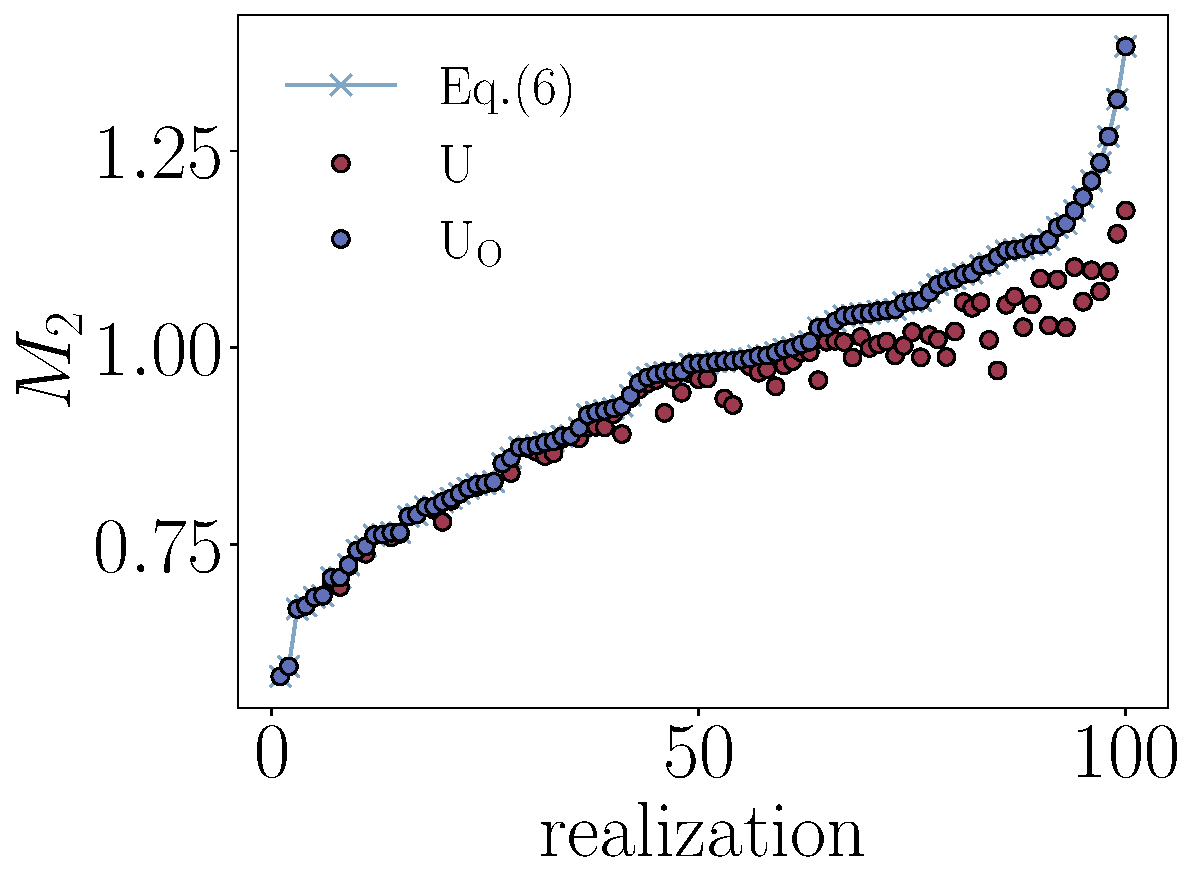
\includegraphics[width=0.9\linewidth]{numerics_5.pdf}};
\begin{scope}[x={(img.south east)},y={(img.north west)}]
\fill[white] (0.362,0.862) rectangle (0.495,0.935);
\node[anchor=west,inner sep=0,font=\small] at (0.368,0.897) {Eq.(\ref*{M-eq:analytic_NL})};
\end{scope}
\end{tikzpicture}
    \caption{Results of the comparison between non-local magic computed with the formula in Eq.~\eqref{M-eq:analytic_NL} (crosses) and the one obtained by minimizing the cost function in Eq.~\eqref{eq:cost_function} with both generic unitaries $U$ (red marker) and fermionic Gaussian unitaries $U_O$ (blue marker), for $100$ different realizations of random fermionic Gaussian states on $N=10$ sites, $\ell=5$. The realizations are ordered by increasing $M_2^{\mathrm{GNL}}$. The formula agrees with minimization over Gaussian unitaries to machine precision in all cases.}
    \label{fig:numerics_verification}
\end{figure}
Instead, in Fig.~\ref{fig:numerics_verification} we show the results of the minimization for $100$ realizations of random Gaussian states on $N=10$ qubits, $\ell=5$, where the minimum is taken both on generic and on fermionic Gaussian unitaries. We also plot the values of Gaussian-restricted non-local magic obtained with our formula for these states, which agree within numerical precision with the results obtained by minimizing over Gaussian unitaries.

A few optimizations were considered in the steps to compute the cost function. When applying the unitaries on the state, it is convenient to reshape the state vector into a $d_A \times d_B$ matrix $\Psi$, such that the application of the unitary $U_A \otimes U_B$ can be computed as $U_A \Psi U_B^{T}$, with reduced cost $\mathcal{O}(d_A^2 d_B + d_A d_B^2)$.
Moreover, the stabilizer entropy of the state vector can be computed using the algorithm introduced in Refs.~\cite{huang2026fastexactapproachstabilizer, sierant2026computingquantummagicstate}, which implements fast Walsh-Hadamard transforms to reduce the time complexity of the computation from $\mathcal{O}(8^N)$ to $\mathcal{O}(N4^N)$, and can also be parallelized for substantial speedup. Finally, the finite-difference method can be replaced with backpropagation, which allows the full $N_p$-dimensional gradient to be computed at a cost comparable to a small constant number of evaluations of the cost function, rather than $O(N_p)$. Note that the number of parameters $N_p$ grows exponentially in $N$ in the case of generic unitaries, and quadratically in $N$ for fermionic Gaussian ones.


\section{Error analysis for experimental accessibility}
\label{app:experimental}
We provide the error propagation analysis connecting the accuracy on $\Gamma_A$ to the accuracy on $M_2^{\mathrm{GNL}}$.
Since $\mathfrak{m}_2(\lambda^2) = -\log_2(1-\lambda^2+\lambda^4)$ is smooth on $[0,1]$, its derivative
\begin{equation}
    \frac{d}{d\lambda}\,\mathfrak{m}_2(\lambda^2) = \frac{2\lambda(1-2\lambda^2)}{(1-\lambda^2+\lambda^4)\ln 2}
\end{equation}
is bounded, so $\mathfrak{m}_2$ is uniformly Lipschitz on $[0,1]$ with constant $L = \max_{\lambda \in [0,1]} \bigl|\frac{d}{d\lambda}\mathfrak{m}_2(\lambda^2)\bigr| = O(1)$.
Combining with the Hoffman--Wielandt stability bound for eigenvalues of $i\Gamma_A$,
\begin{equation}
    |\delta M_2^{\mathrm{GNL}}| \lesssim L\,\sqrt{\ell}\,\|\delta\Gamma_A\|_F\;.
\end{equation}
A uniform entrywise error $\epsilon_\Gamma$ implies $\|\delta\Gamma_A\|_F = O(\ell \epsilon_\Gamma)$, giving $|\delta M_2^{\mathrm{GNL}}| = \mathcal{O}(\ell^{3/2}\epsilon_\Gamma)$.
To estimate the non-local magic density $m_2^{\mathrm{GNL}} = M_2^{\mathrm{GNL}}/\ell$ with additive accuracy $\varepsilon$, one needs $\epsilon_\Gamma = \mathcal{O}(\varepsilon/\sqrt{\ell})$, yielding
\begin{equation}
    N_{\mathrm{shots}} = O\!\left(\frac{\ell^3\log(\ell/\delta)}{\varepsilon^2}\right).
\end{equation}
This estimate is pessimistic for gapped phases, where $\Gamma_A$ is approximately banded and only $\mathcal{O}(1)$ entanglement modes near the boundary contribute appreciably; near criticality the bound is closer to the true cost.

\section{$\alpha$-Generalization of Results}
\label{Sec:generaliz}

In the main text, several results were discussed exclusively for the Rényi index $\alpha = 2$. For completeness, we now present their extensions to arbitrary integer $\alpha \ge 2$. These extensions are obtained from the conjectured weights of Eq.~\eqref{M-eq:analytic_NL_alpha}; at $\alpha=2$ they reduce to the results of the main text, which follow from Theorem~\ref{M-thm:global}.

We begin with the Page curve. From Eq.~\eqref{M-eq:ziopin2}, replacing $\mathfrak{m}_2$ with $\mathfrak{m}_\alpha$, we find that the behavior for $r \simeq 0$ remains the same for every $\alpha$ up to a constant:
\begin{equation}
\overline{\mathsf{m}}_\alpha(r \simeq 0) = - \frac{\alpha}{1-\alpha} \frac{r^2}{2 \ln 2} + O(r^3).
\end{equation}

Next, we consider the critical behavior in the Ising model. From Eq.~\eqref{M-eq:alpha_NL}, substituting $\mathfrak{m}_2 \mapsto \mathfrak{m}_\alpha$, a change of variables $\lambda = \frac{1-t}{1+t}$ leads to
\begin{equation}
\beta_{\mathrm{GNL}}(\alpha) = \frac{1}{\pi^2 (1-\alpha) \ln 2} \int_0^1 \frac{\hat{\mathfrak{m}}_\alpha(t)}{t}\, dt,
\end{equation}
where
\begin{equation}
\hat{\mathfrak{m}}_\alpha(t) = \ln \left[ \frac{(1+t)^{2\alpha} + (1-t)^{2\alpha} + 4^\alpha t^\alpha}{2 (1+t)^{2\alpha}} \right].
\end{equation}
Noting that $\hat{\mathfrak{m}}_\alpha(t) = \hat{\mathfrak{m}}_\alpha(1/t)$, the integral can equivalently be written as
\begin{equation}
\beta_{\mathrm{GNL}}(\alpha) = \frac{1}{2 \pi^2 (1-\alpha) \ln 2} \int_0^\infty \frac{\hat{\mathfrak{m}}_\alpha(t)}{t}\, dt,
\end{equation} 
which corresponds to the Mellin transform of $\hat{\mathfrak{m}}_\alpha(t)$ evaluated as $s \to 0$.
The result of the integral is given by 
\begin{equation}
\beta_{\mathrm{GNL}}(\alpha) = \frac{1}{2 (1-\alpha) \pi^2 \ln(2)}\sum_{j=1}^\alpha \mathrm{arccosh}^2(-r_j/2)\;,
\end{equation}
where $r_j$ are the (generally complex) roots of the polynomial $R_\alpha(x)=(x-2)^\alpha+(x+2)^\alpha+4^\alpha$.

\section{Details on the numerical simulations}
\label{app:numerics}

\subsection{SYK$_2$ mid-spectrum eigenstates}
\label{app:syk}
The SYK$_2$ model is specified by the Hamiltonian  $H$ of the form in  Eq.~\eqref{M-eq:ham} with  $h$ a random antisymmetric matrix whose elements are drawn from the normal distribution $h_{m,n}\sim \mathcal{N}(0,{J^2}/{N})$ and set $J=1$. 
The single-body Hamiltonian $ih$ is Hermitian with eigenvalues in $\pm\varepsilon_k$ pairs ($k=1,\dots,N$), each pair defining an effective fermionic mode. A many-body eigenstate is specified by a filling $\mathcal{F}\subset\{1,\dots,2N\}$ of $N$ single-particle modes with eigenvectors $|v_k\rangle$, yielding the one-body density matrix $\Xi=\sum_{k\in\mathcal{F}}|v_k\rangle\langle v_k|$ and the covariance matrix $\Gamma = i(2\Xi-\mathbb{I})$. 
The ground state fills the $N$ lowest-energy modes; to probe typicality, we construct mid-spectrum eigenstates $H|E_n\rangle=E_n|E_n\rangle$  by flipping a random subset of $N/4$ to $N/2$ modes from the ground-state configuration, replacing occupied negative-energy modes with their positive-energy partners. For each of $N_{\mathrm{dis}}=1000$ disorder realizations, we compute $M_2^{\mathrm{GNL}}$ from $\Gamma$ and average over 200 excited eigenstates $|E_n\rangle$ per realization, obtaining $\overline{M}_2^{\mathrm{GNL}}=\mathbb{E}_{h}\,\mathbb{E}_{n}[M_2^{\mathrm{GNL}}(|E_n\rangle)]$.
In Fig.~\ref{M-fig:typicality}(b), we plot the resulting non-local magic density $\overline{\mathsf{m}}_2^\mathrm{GNL}$ versus $r=\ell/N$ for $N=40,80,160$.

\subsection{Random Gaussian circuits}
\label{app:circuits}
The circuit is composed of nearest-neighbor fermionic Gaussian unitaries arranged in a brick-wall geometry on $N$ sites.
A single layer $O_{\mathrm{layer}} = O_{\mathrm{odd}}\,O_{\mathrm{even}}$ consists of an even and an odd half-step, namely $O_{\mathrm{even}} = \prod_{j=1}^{N/2} R_{2j-1,2j}$ and $O_{\mathrm{odd}} = \prod_{j=1}^{N/2-1} R_{2j,2j+1}$, where each $R_{j,j+1} \in \mathrm{SO}(4)$ is a random orthogonal matrix drawn independently from the Haar measure, acting on the four Majorana operators $(\gamma_{2j-1}, \gamma_{2j}, \gamma_{2j+1}, \gamma_{2j+2})$ of sites $j$ and $j+1$.
The full circuit after $t$ layers is $O(t) = \prod_{s=1}^t O_{\mathrm{layer}}^{(s)} \in \mathrm{SO}(2N)$.
The initial state is the product state $|\mathbf{0}\rangle$ (vacuum of all fermionic modes), with covariance matrix $\Gamma_0$. 

The time-evolved state remains Gaussian at all times, with covariance matrix $\Gamma(t) = O(t)\,\Gamma_0\,O(t)^T$.
The Gaussian-restricted non-local magic is therefore entirely determined by the restricted covariance matrix $\Gamma_A(t)$ and its eigenvalues $\pm\lambda_j(t)$.


\bibliography{ref_current}

\end{document}
